\section{Задание 1. Непрерывные динамические системы}

В данном задании мы исследуем непрерывные динамические системы второго порядка вида:
\begin{equation}
\dot{x}(t) = Ax(t), \quad x(t) \in \mathbb{R}^2, \quad A \in \mathbb{R}^{2 \times 2}
\end{equation}

Зададим два неколлинеарных вектора, не лежащих на координатных осях:
\begin{equation}
v_1 = \begin{pmatrix} 1 \\ 1 \end{pmatrix}, \quad v_2 = \begin{pmatrix} -1 \\ 2 \end{pmatrix}
\end{equation}

Проверим, что векторы неколлинеарны:
\begin{equation}
\det([v_1, v_2]) = \begin{vmatrix} 1 & -1 \\ 1 & 2 \end{vmatrix} = 1 \cdot 2 - 1 \cdot (-1) = 2 + 1 = 3 \neq 0
\end{equation}

\subsection{Система 1: Асимптотически устойчивая система}

Создадим систему, которая асимптотически устойчива, при этом если $x(0) = v_1$, то $x(t) \in \text{Span}\{v_1\}$, а если $x(0) = v_2$, то $x(t) \in \text{Span}\{v_2\}$ при всех $t \geq 0$.

Для этого нужно найти матрицу $A$ такую, что $Av_1 = \lambda_1 v_1$ и $Av_2 = \lambda_2 v_2$, где $\lambda_1, \lambda_2 < 0$.

Пусть $\lambda_1 = -1$, $\lambda_2 = -2$. Решаем систему уравнений:
\begin{align}
A \begin{pmatrix} 1 \\ 1 \end{pmatrix} &= -1 \begin{pmatrix} 1 \\ 1 \end{pmatrix} \\
A \begin{pmatrix} -1 \\ 2 \end{pmatrix} &= -2 \begin{pmatrix} -1 \\ 2 \end{pmatrix}
\end{align}

Получаем матрицу:
\begin{equation}
A_1 = \begin{pmatrix} -\frac{4}{3} & \frac{1}{3} \\ \frac{2}{3} & -\frac{5}{3} \end{pmatrix}
\end{equation}

Собственные значения: $\lambda_1 = -1$, $\lambda_2 = -2$

Собственные векторы:
\begin{equation}
v_1 = \begin{pmatrix} 1 \\ 1 \end{pmatrix}, \quad v_2 = \begin{pmatrix} -1 \\ 2 \end{pmatrix}
\end{equation}

\subsection{Система 2: Неустойчивая система без неколлинеарных собственных векторов}

Используем жорданову клетку:
\begin{equation}
A_2 = \begin{pmatrix} -1 & 1 \\ 0 & -1 \end{pmatrix}
\end{equation}

Собственные значения: $\lambda_1 = \lambda_2 = -1$ (кратное)

Собственные векторы: только один линейно независимый вектор $\begin{pmatrix} 1 \\ 0 \end{pmatrix}$

\subsection{Система 3: Неустойчивая система с особым поведением}

Используем диагональную матрицу с разными знаками собственных значений:
\begin{equation}
A_3 = \begin{pmatrix} 1 & 0 \\ 0 & -2 \end{pmatrix}
\end{equation}

Собственные значения: $\lambda_1 = 1$, $\lambda_2 = -2$

Собственные векторы:
\begin{equation}
v_1 = \begin{pmatrix} 1 \\ 0 \end{pmatrix}, \quad v_2 = \begin{pmatrix} 0 \\ 1 \end{pmatrix}
\end{equation}

Если $x(0) = v_2$, то $x(t) = e^{-2t}v_2 \to 0$ при $t \to \infty$.

\subsection{Система 4: Асимптотически устойчивая система с комплексными собственными векторами}

Используем матрицу с комплексными собственными значениями с отрицательной вещественной частью:
\begin{equation}
A_4 = \begin{pmatrix} -1 & -1 \\ 1 & -1 \end{pmatrix}
\end{equation}

Собственные значения: $\lambda_1 = -1 + i$, $\lambda_2 = -1 - i$

Собственные векторы (комплексные):
\begin{equation}
v_1 = \begin{pmatrix} 1 \\ -i \end{pmatrix}, \quad v_2 = \begin{pmatrix} 1 \\ i \end{pmatrix}
\end{equation}

\subsection{Система 5: Неустойчивая система с комплексными собственными векторами}

Используем ту же структуру, но с положительной вещественной частью:
\begin{equation}
A_5 = \begin{pmatrix} 1 & -1 \\ 1 & 1 \end{pmatrix}
\end{equation}

Собственные значения: $\lambda_1 = 1 + i$, $\lambda_2 = 1 - i$

Собственные векторы (комплексные):
\begin{equation}
v_1 = \begin{pmatrix} 1 \\ -i \end{pmatrix}, \quad v_2 = \begin{pmatrix} 1 \\ i \end{pmatrix}
\end{equation}

\subsection{Система 6: Нейтрально устойчивая система}

Используем мнимые собственные значения:
\begin{equation}
A_6 = \begin{pmatrix} 0 & -1 \\ 1 & 0 \end{pmatrix}
\end{equation}

Собственные значения: $\lambda_1 = i$, $\lambda_2 = -i$

Собственные векторы (комплексные):
\begin{equation}
v_1 = \begin{pmatrix} 1 \\ -i \end{pmatrix}, \quad v_2 = \begin{pmatrix} 1 \\ i \end{pmatrix}
\end{equation}

\subsection{Моделирование непрерывных систем}

На рис. \ref{fig:continuous_systems} представлены графики для всех шести систем с различными начальными условиями.

\begin{figure}[h!]
\centering
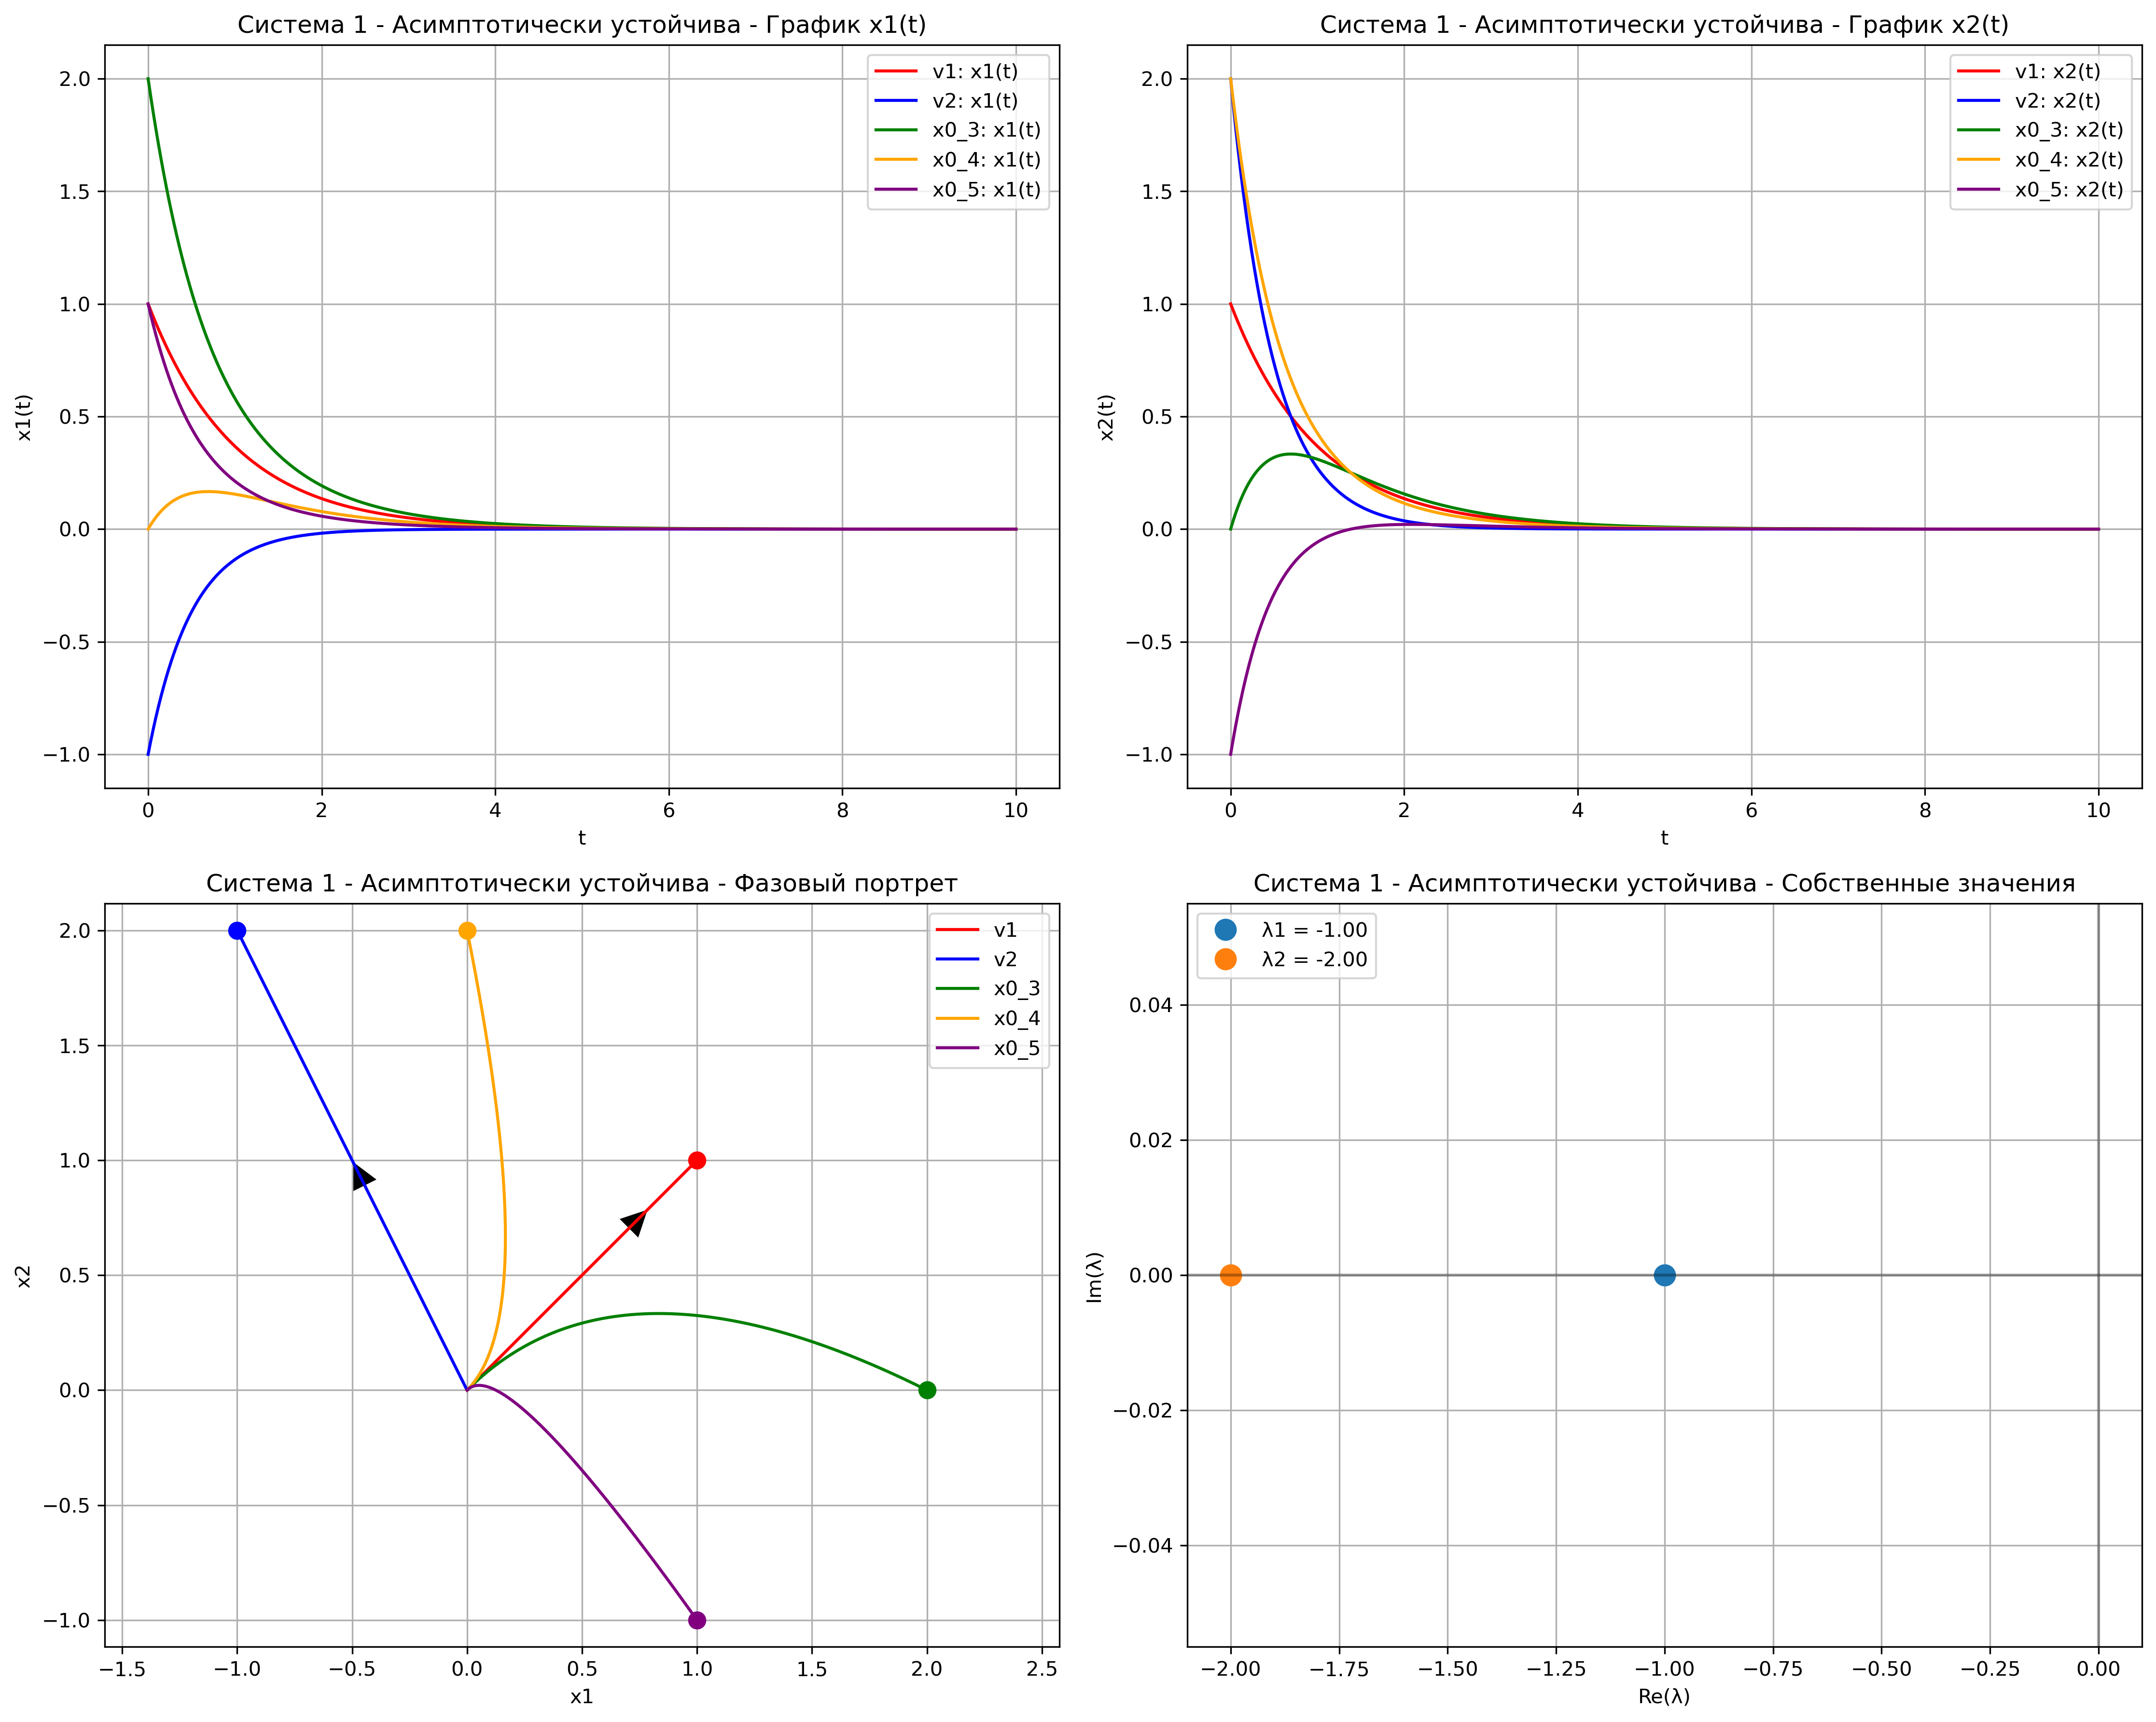
\includegraphics[width=0.8\textwidth]{images/task1/система_1_-_асимптотически_устойчива.png}
\caption{Система 1: Асимптотически устойчивая система}
\label{fig:system1}
\end{figure}

\begin{figure}[h!]
\centering
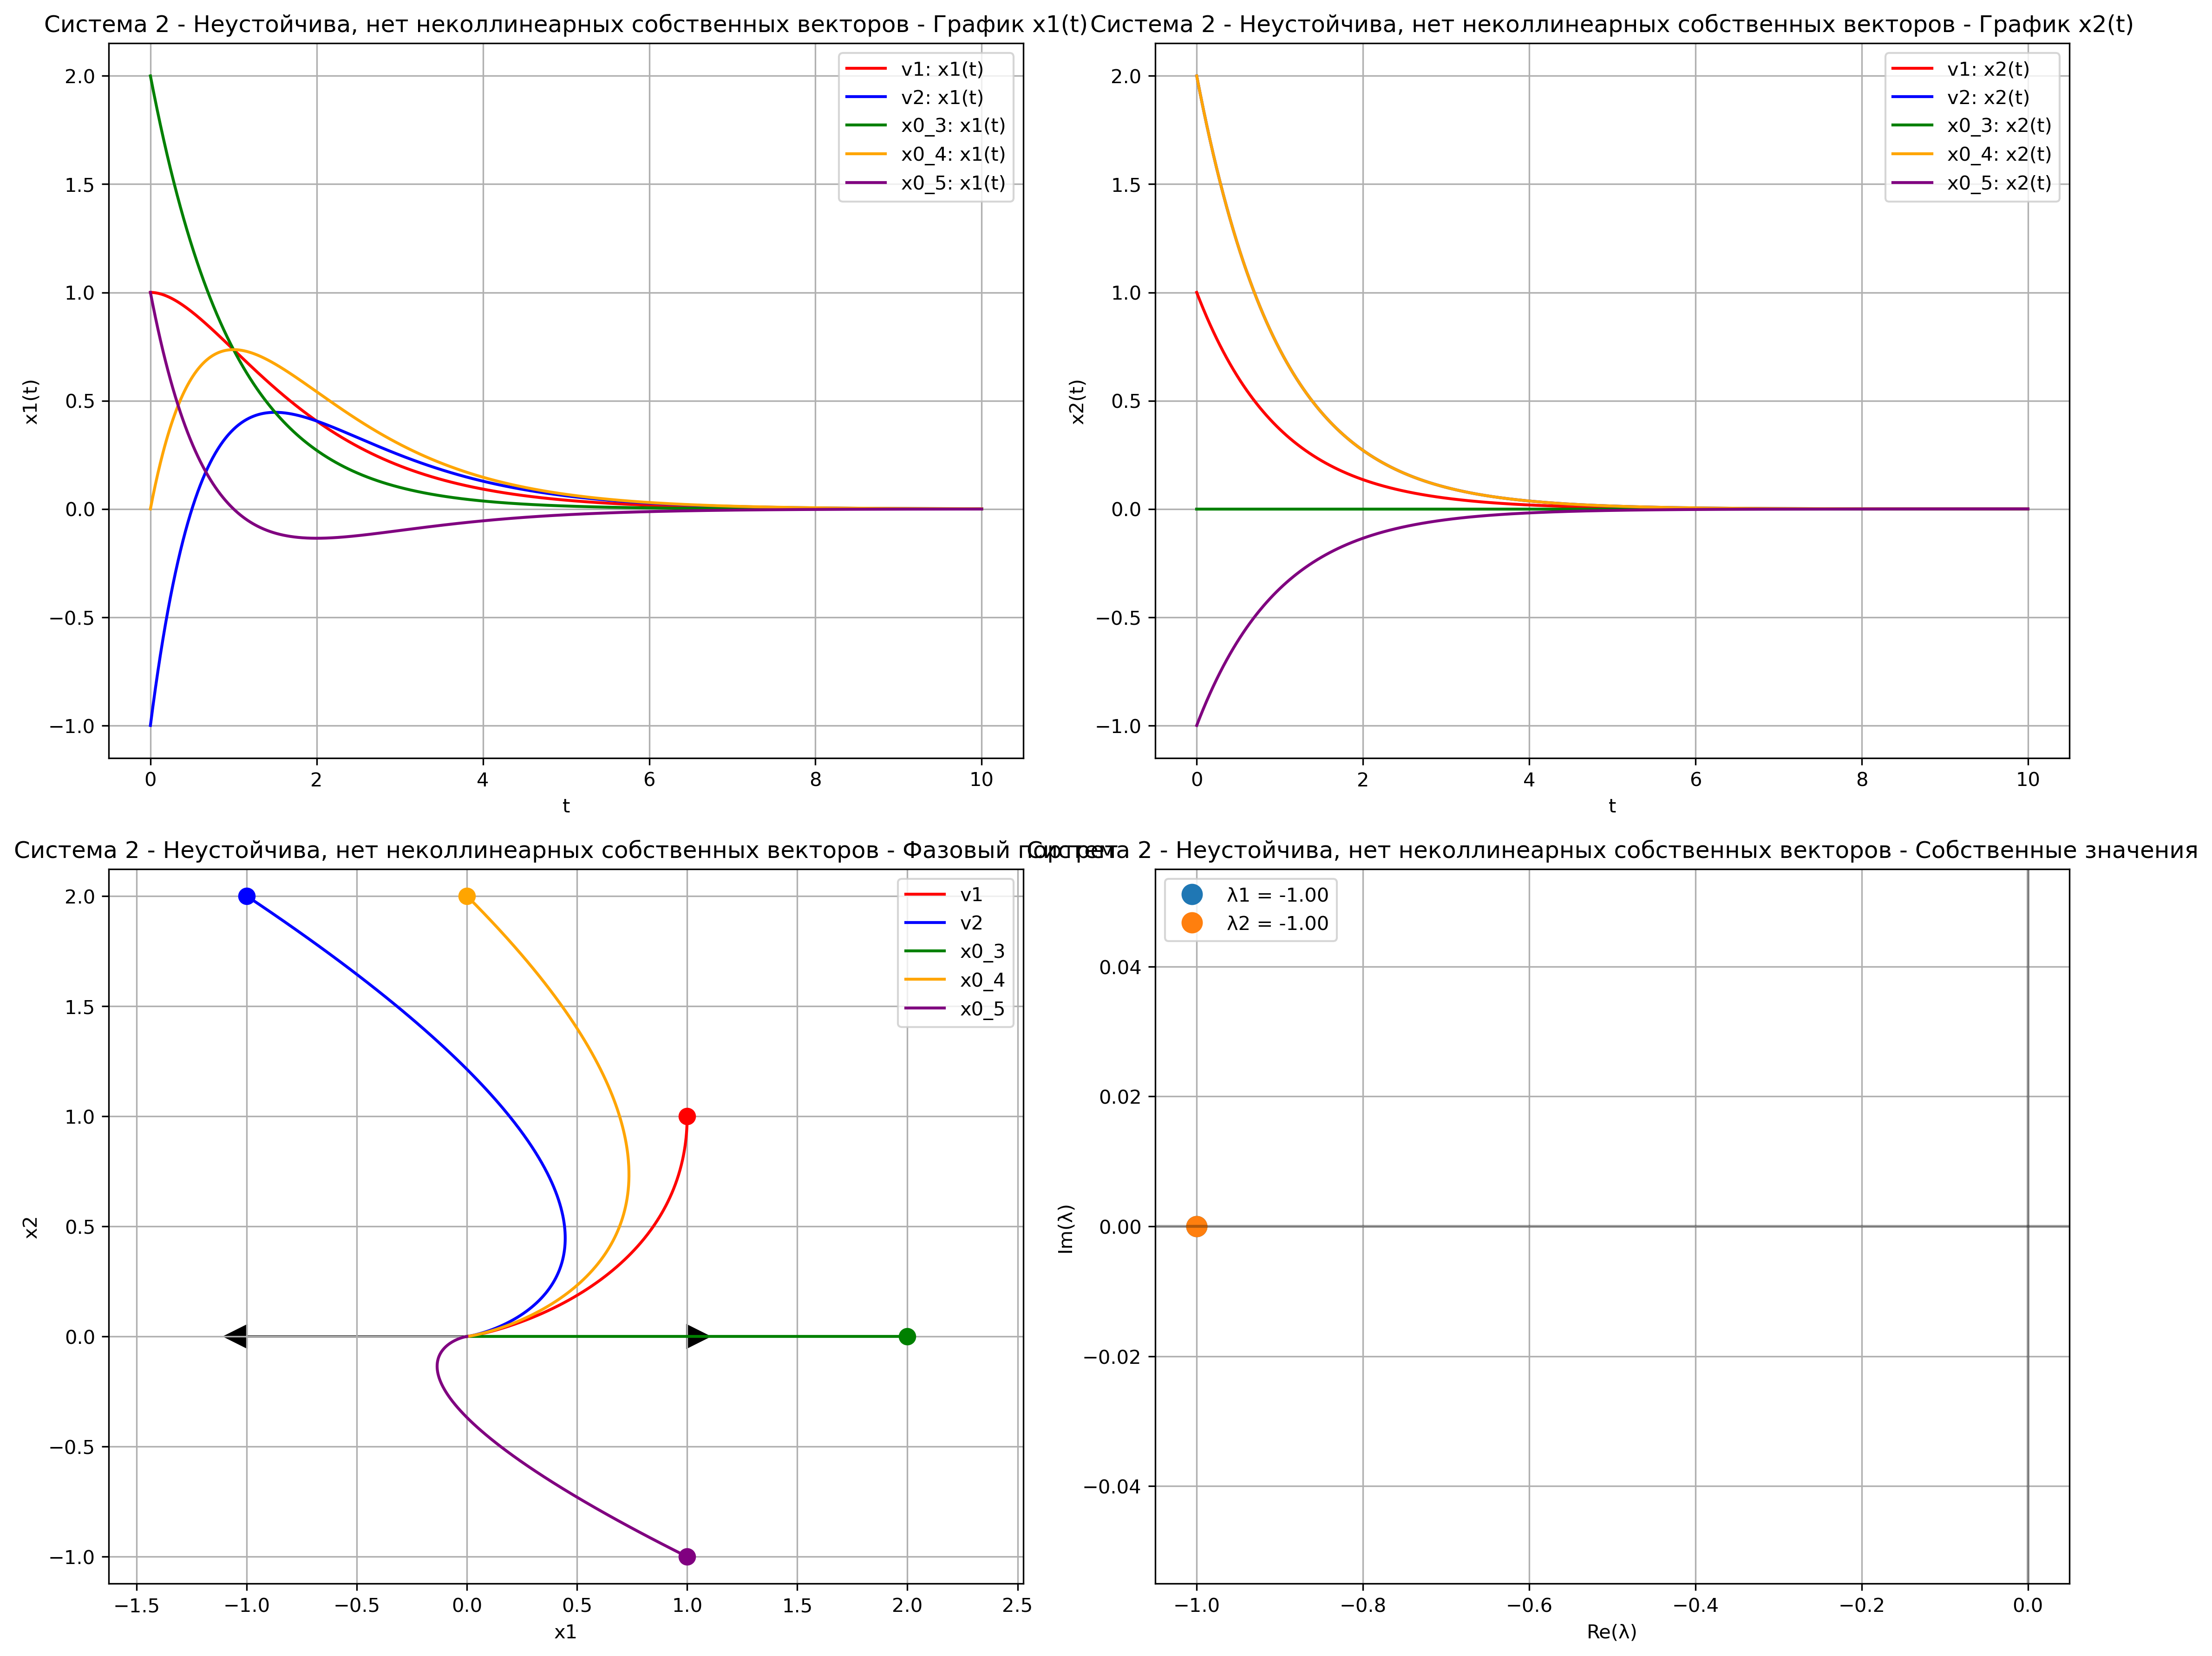
\includegraphics[width=0.8\textwidth]{images/task1/система_2_-_неустойчива,_нет_неколлинеарных_собственных_векторов.png}
\caption{Система 2: Неустойчивая система без неколлинеарных собственных векторов}
\label{fig:system2}
\end{figure}

\begin{figure}[h!]
\centering
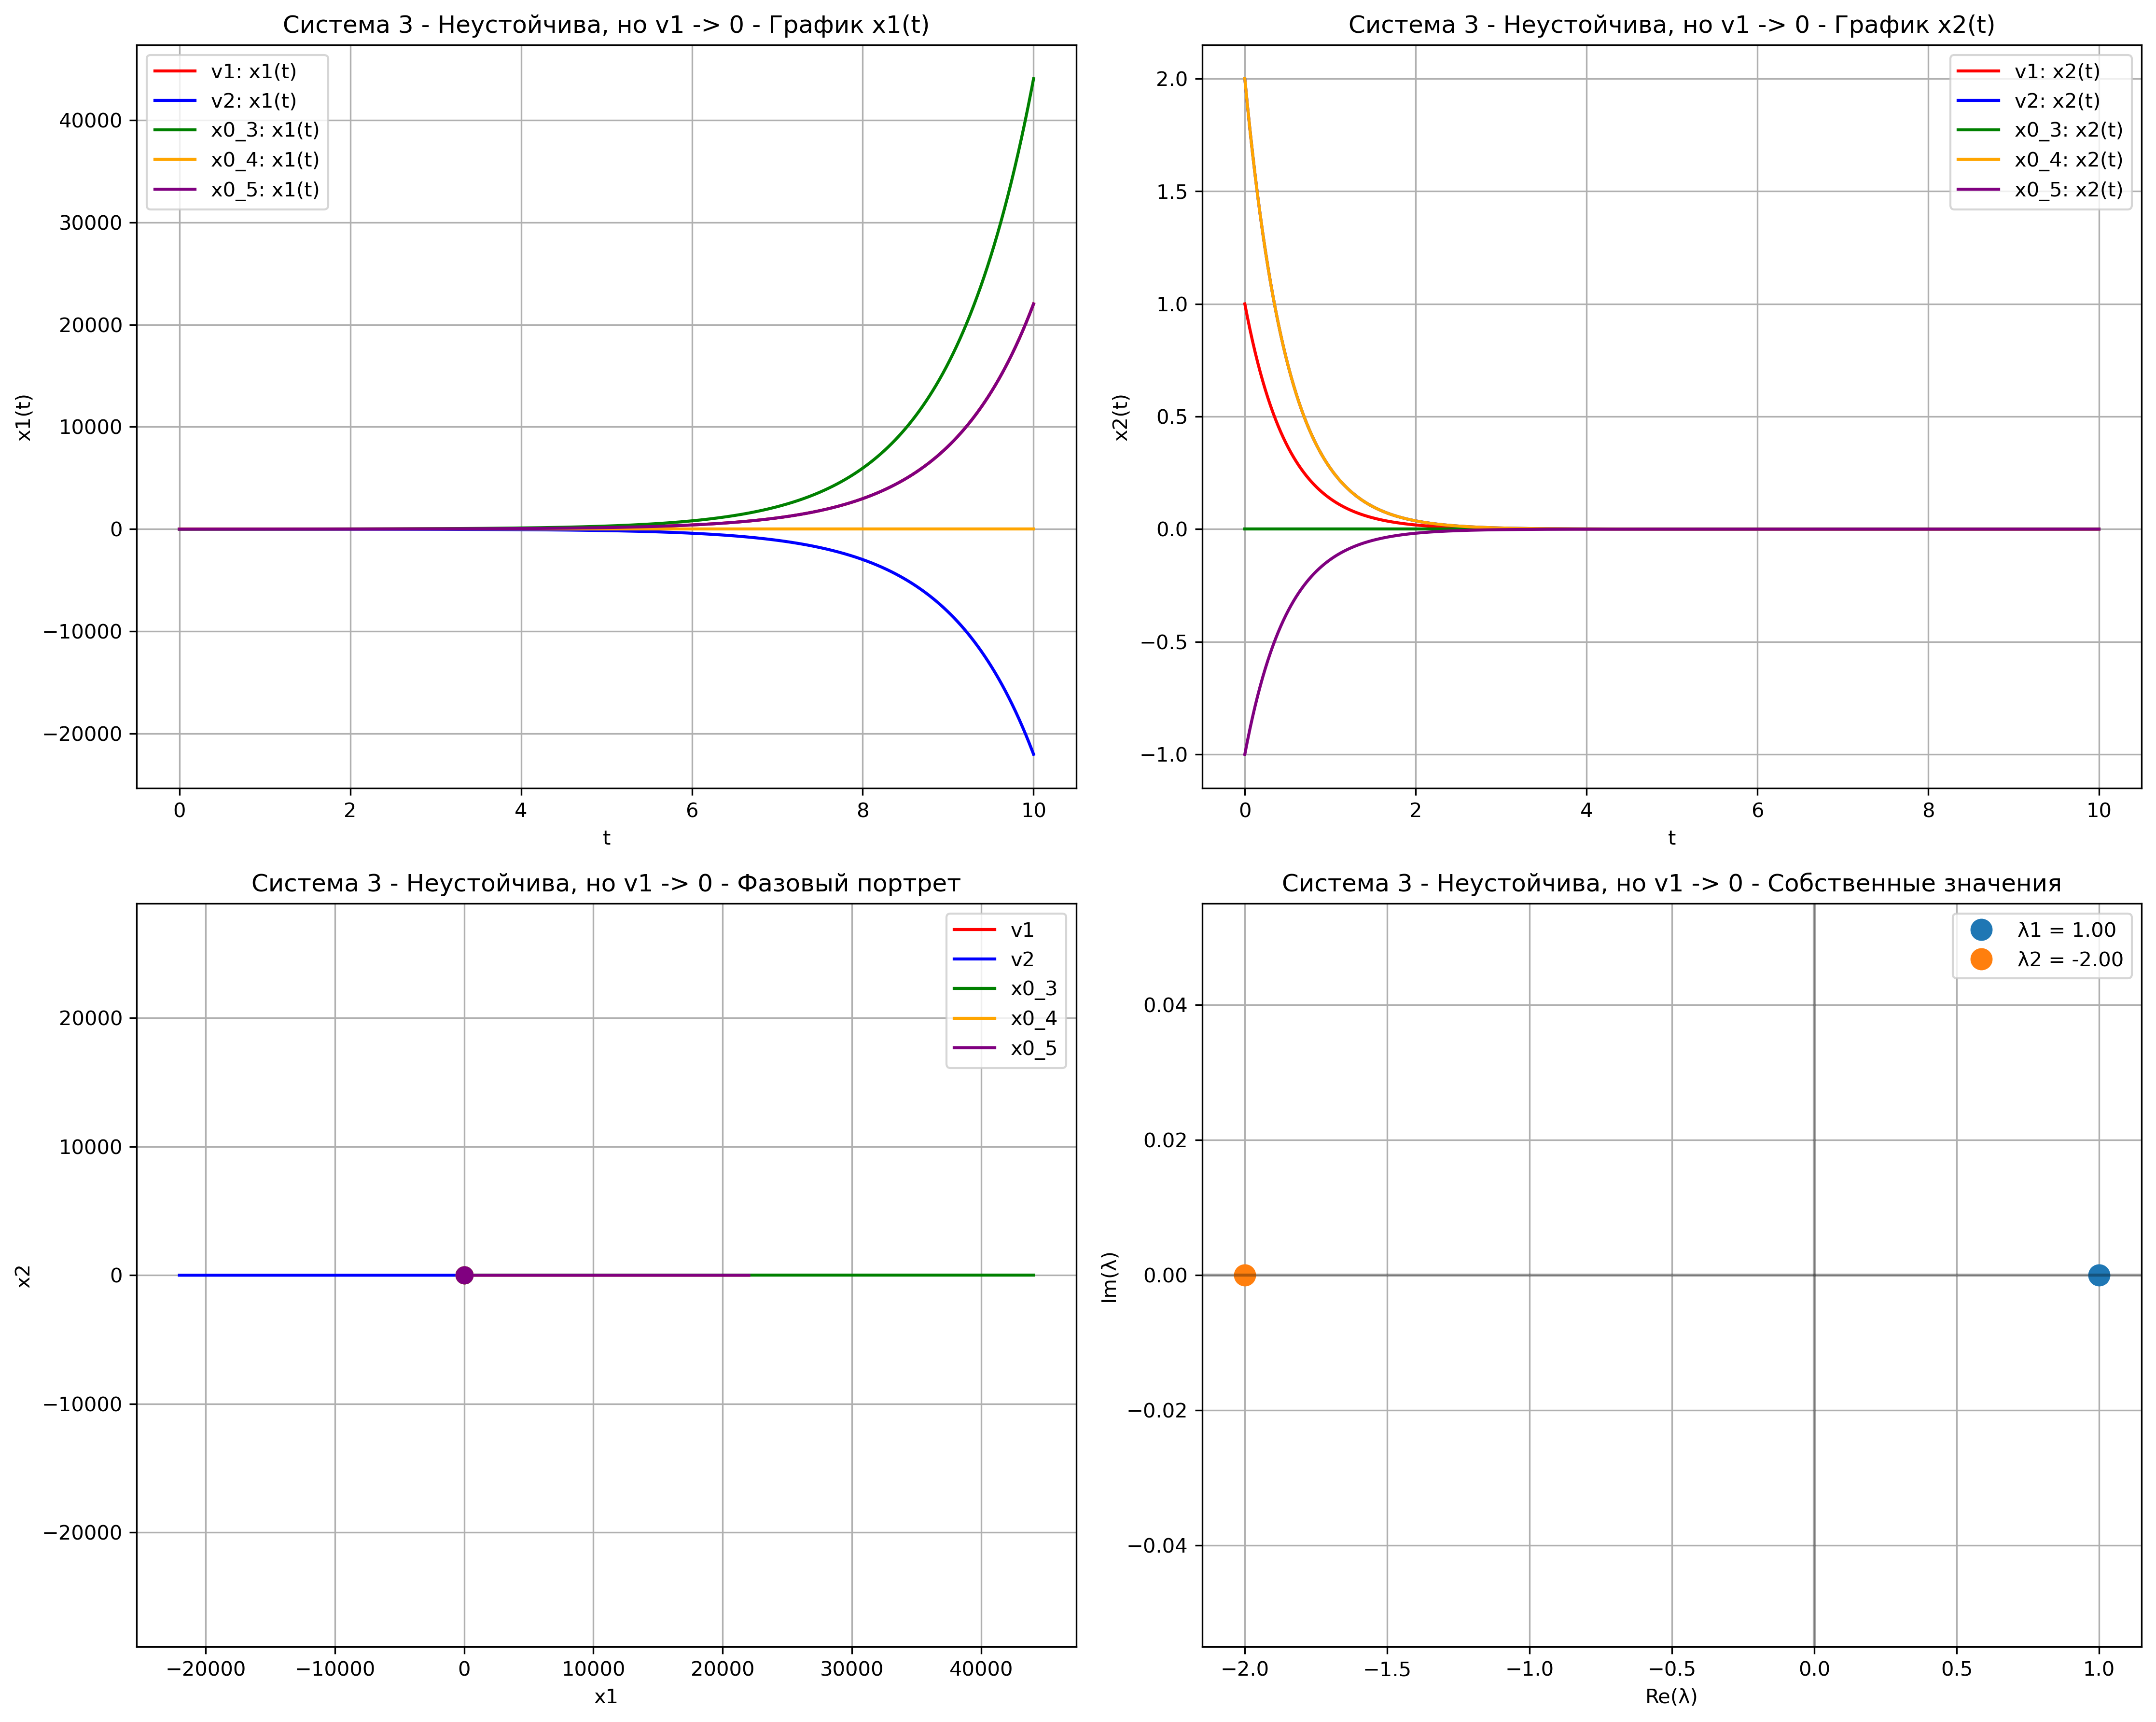
\includegraphics[width=0.8\textwidth]{images/task1/система_3_-_неустойчива,_но_v1_->_0.png}
\caption{Система 3: Неустойчивая система с особым поведением}
\label{fig:system3}
\end{figure}

\begin{figure}[h!]
\centering
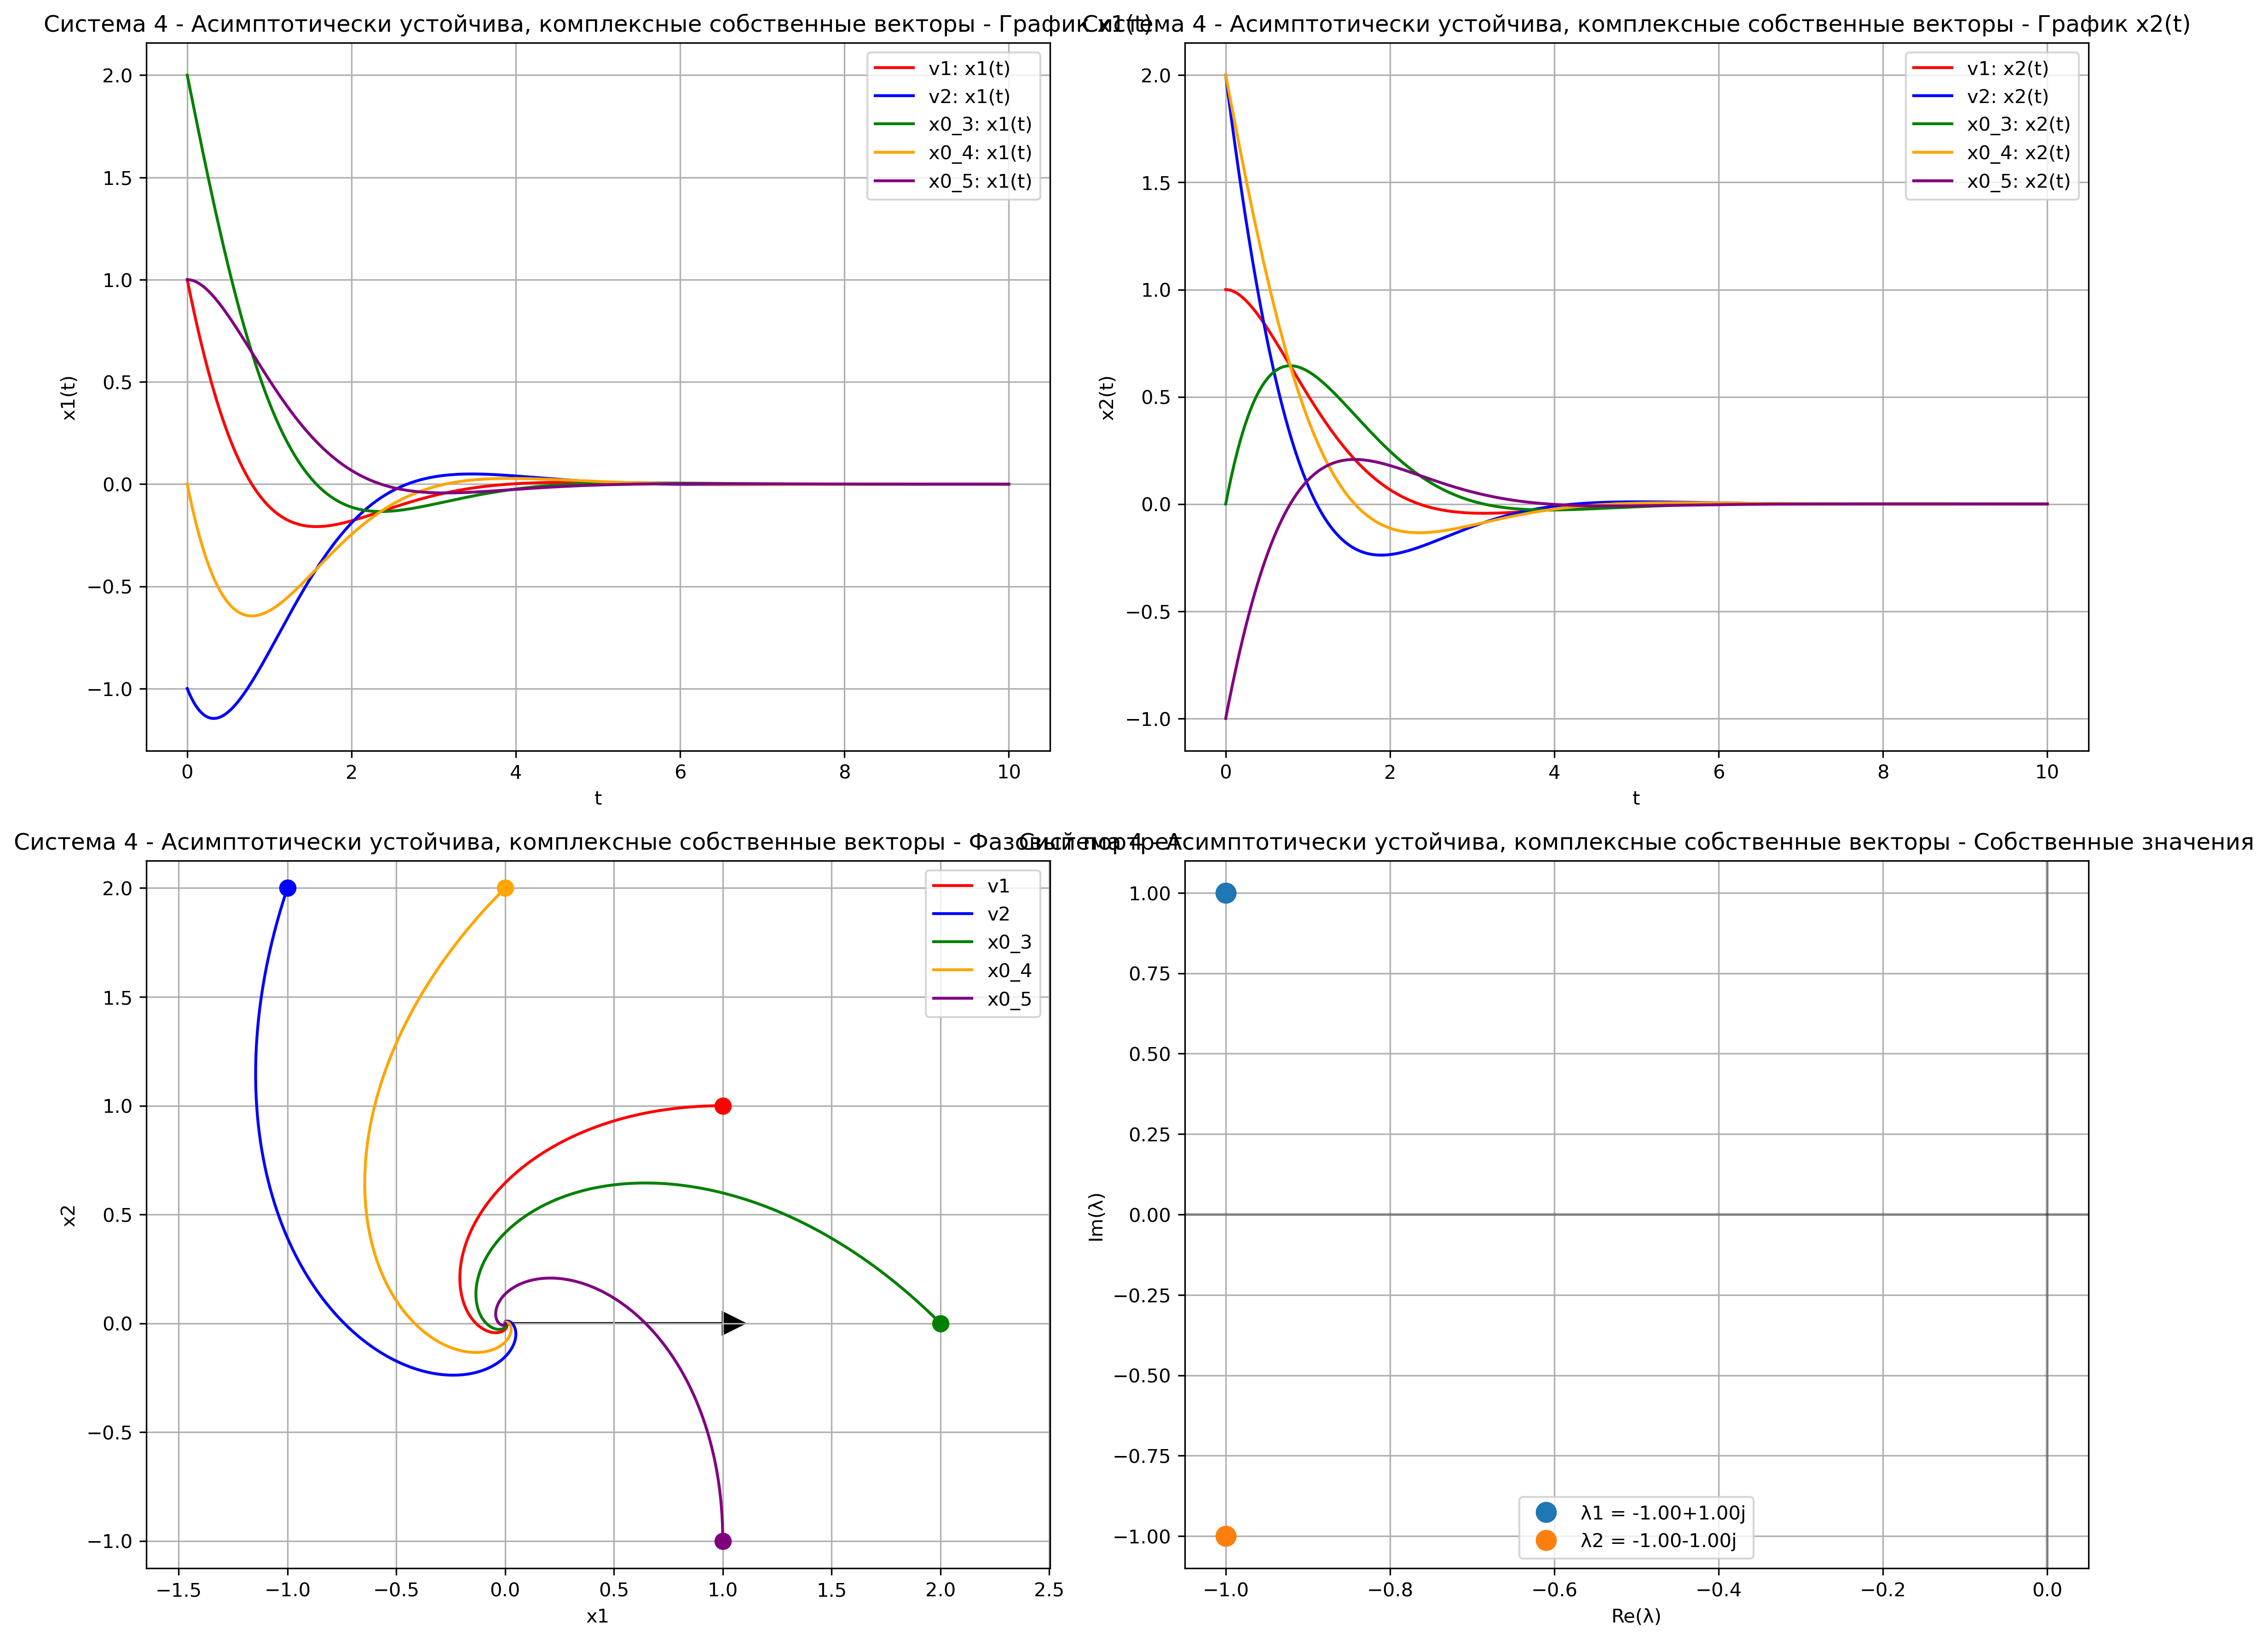
\includegraphics[width=0.8\textwidth]{images/task1/система_4_-_асимптотически_устойчива,_комплексные_собственные_векторы.png}
\caption{Система 4: Асимптотически устойчивая система с комплексными собственными векторами}
\label{fig:system4}
\end{figure}

\begin{figure}[h!]
\centering
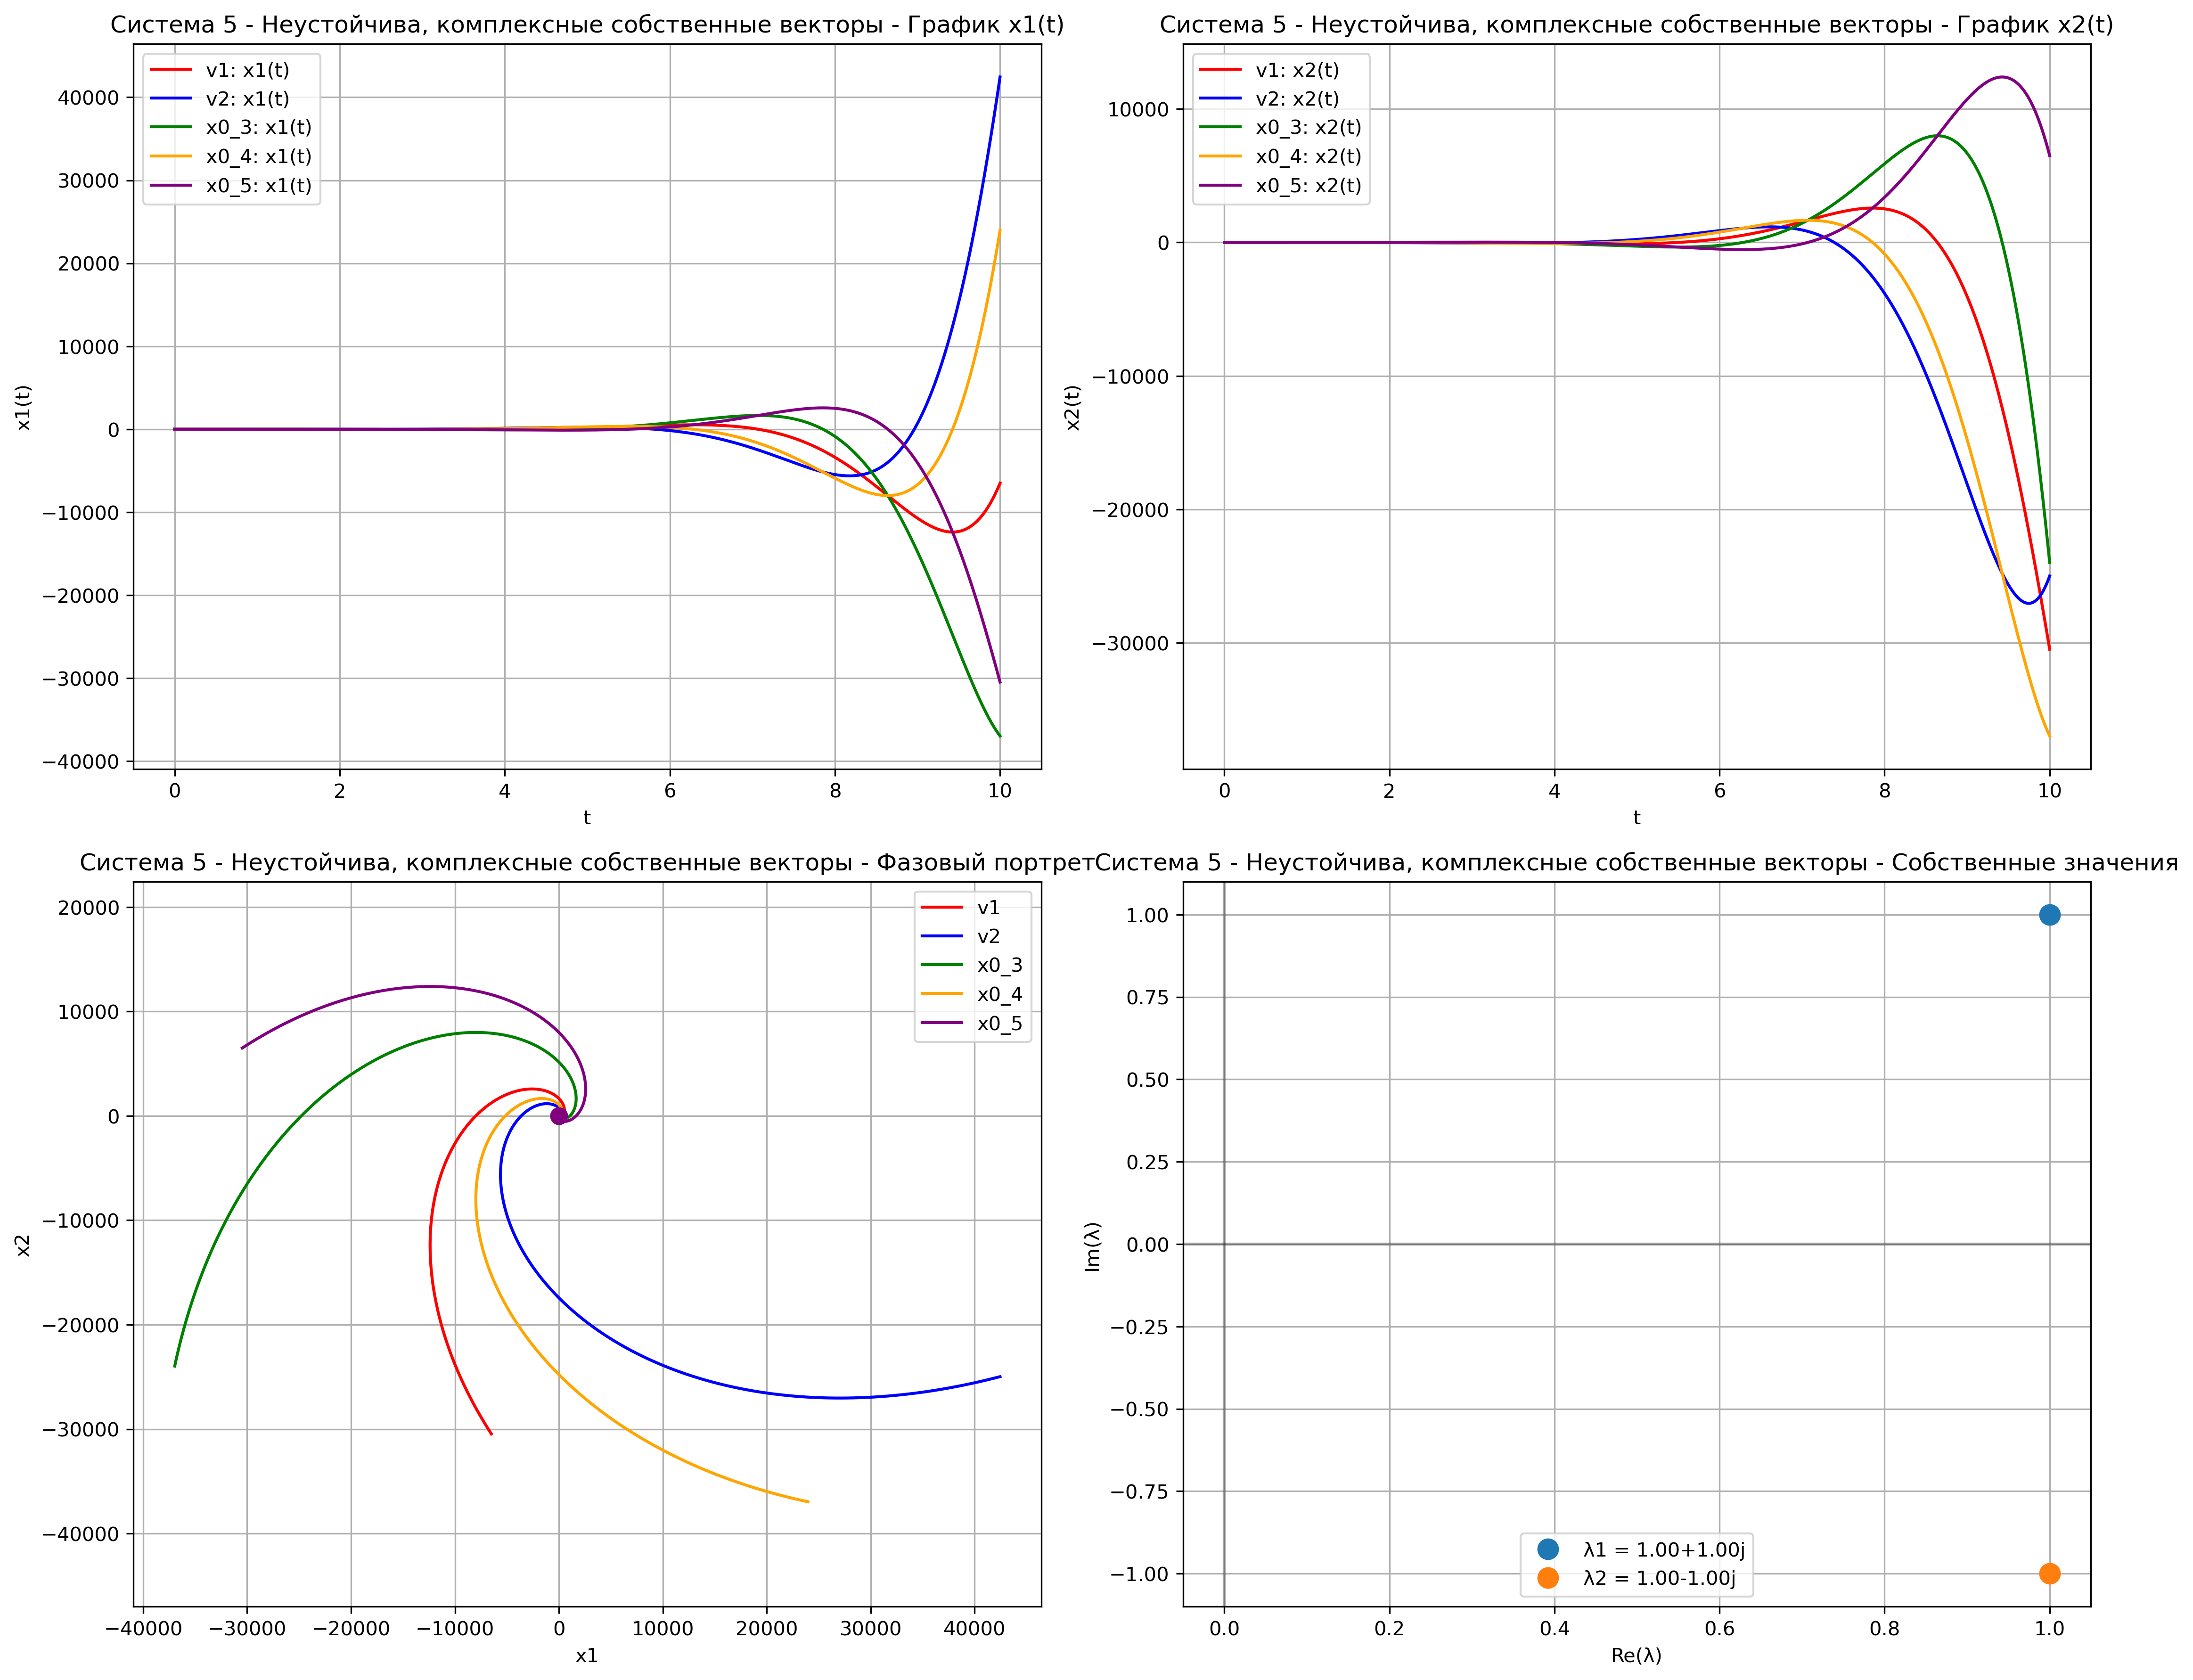
\includegraphics[width=0.8\textwidth]{images/task1/система_5_-_неустойчива,_комплексные_собственные_векторы.png}
\caption{Система 5: Неустойчивая система с комплексными собственными векторами}
\label{fig:system5}
\end{figure}

\begin{figure}[h!]
\centering
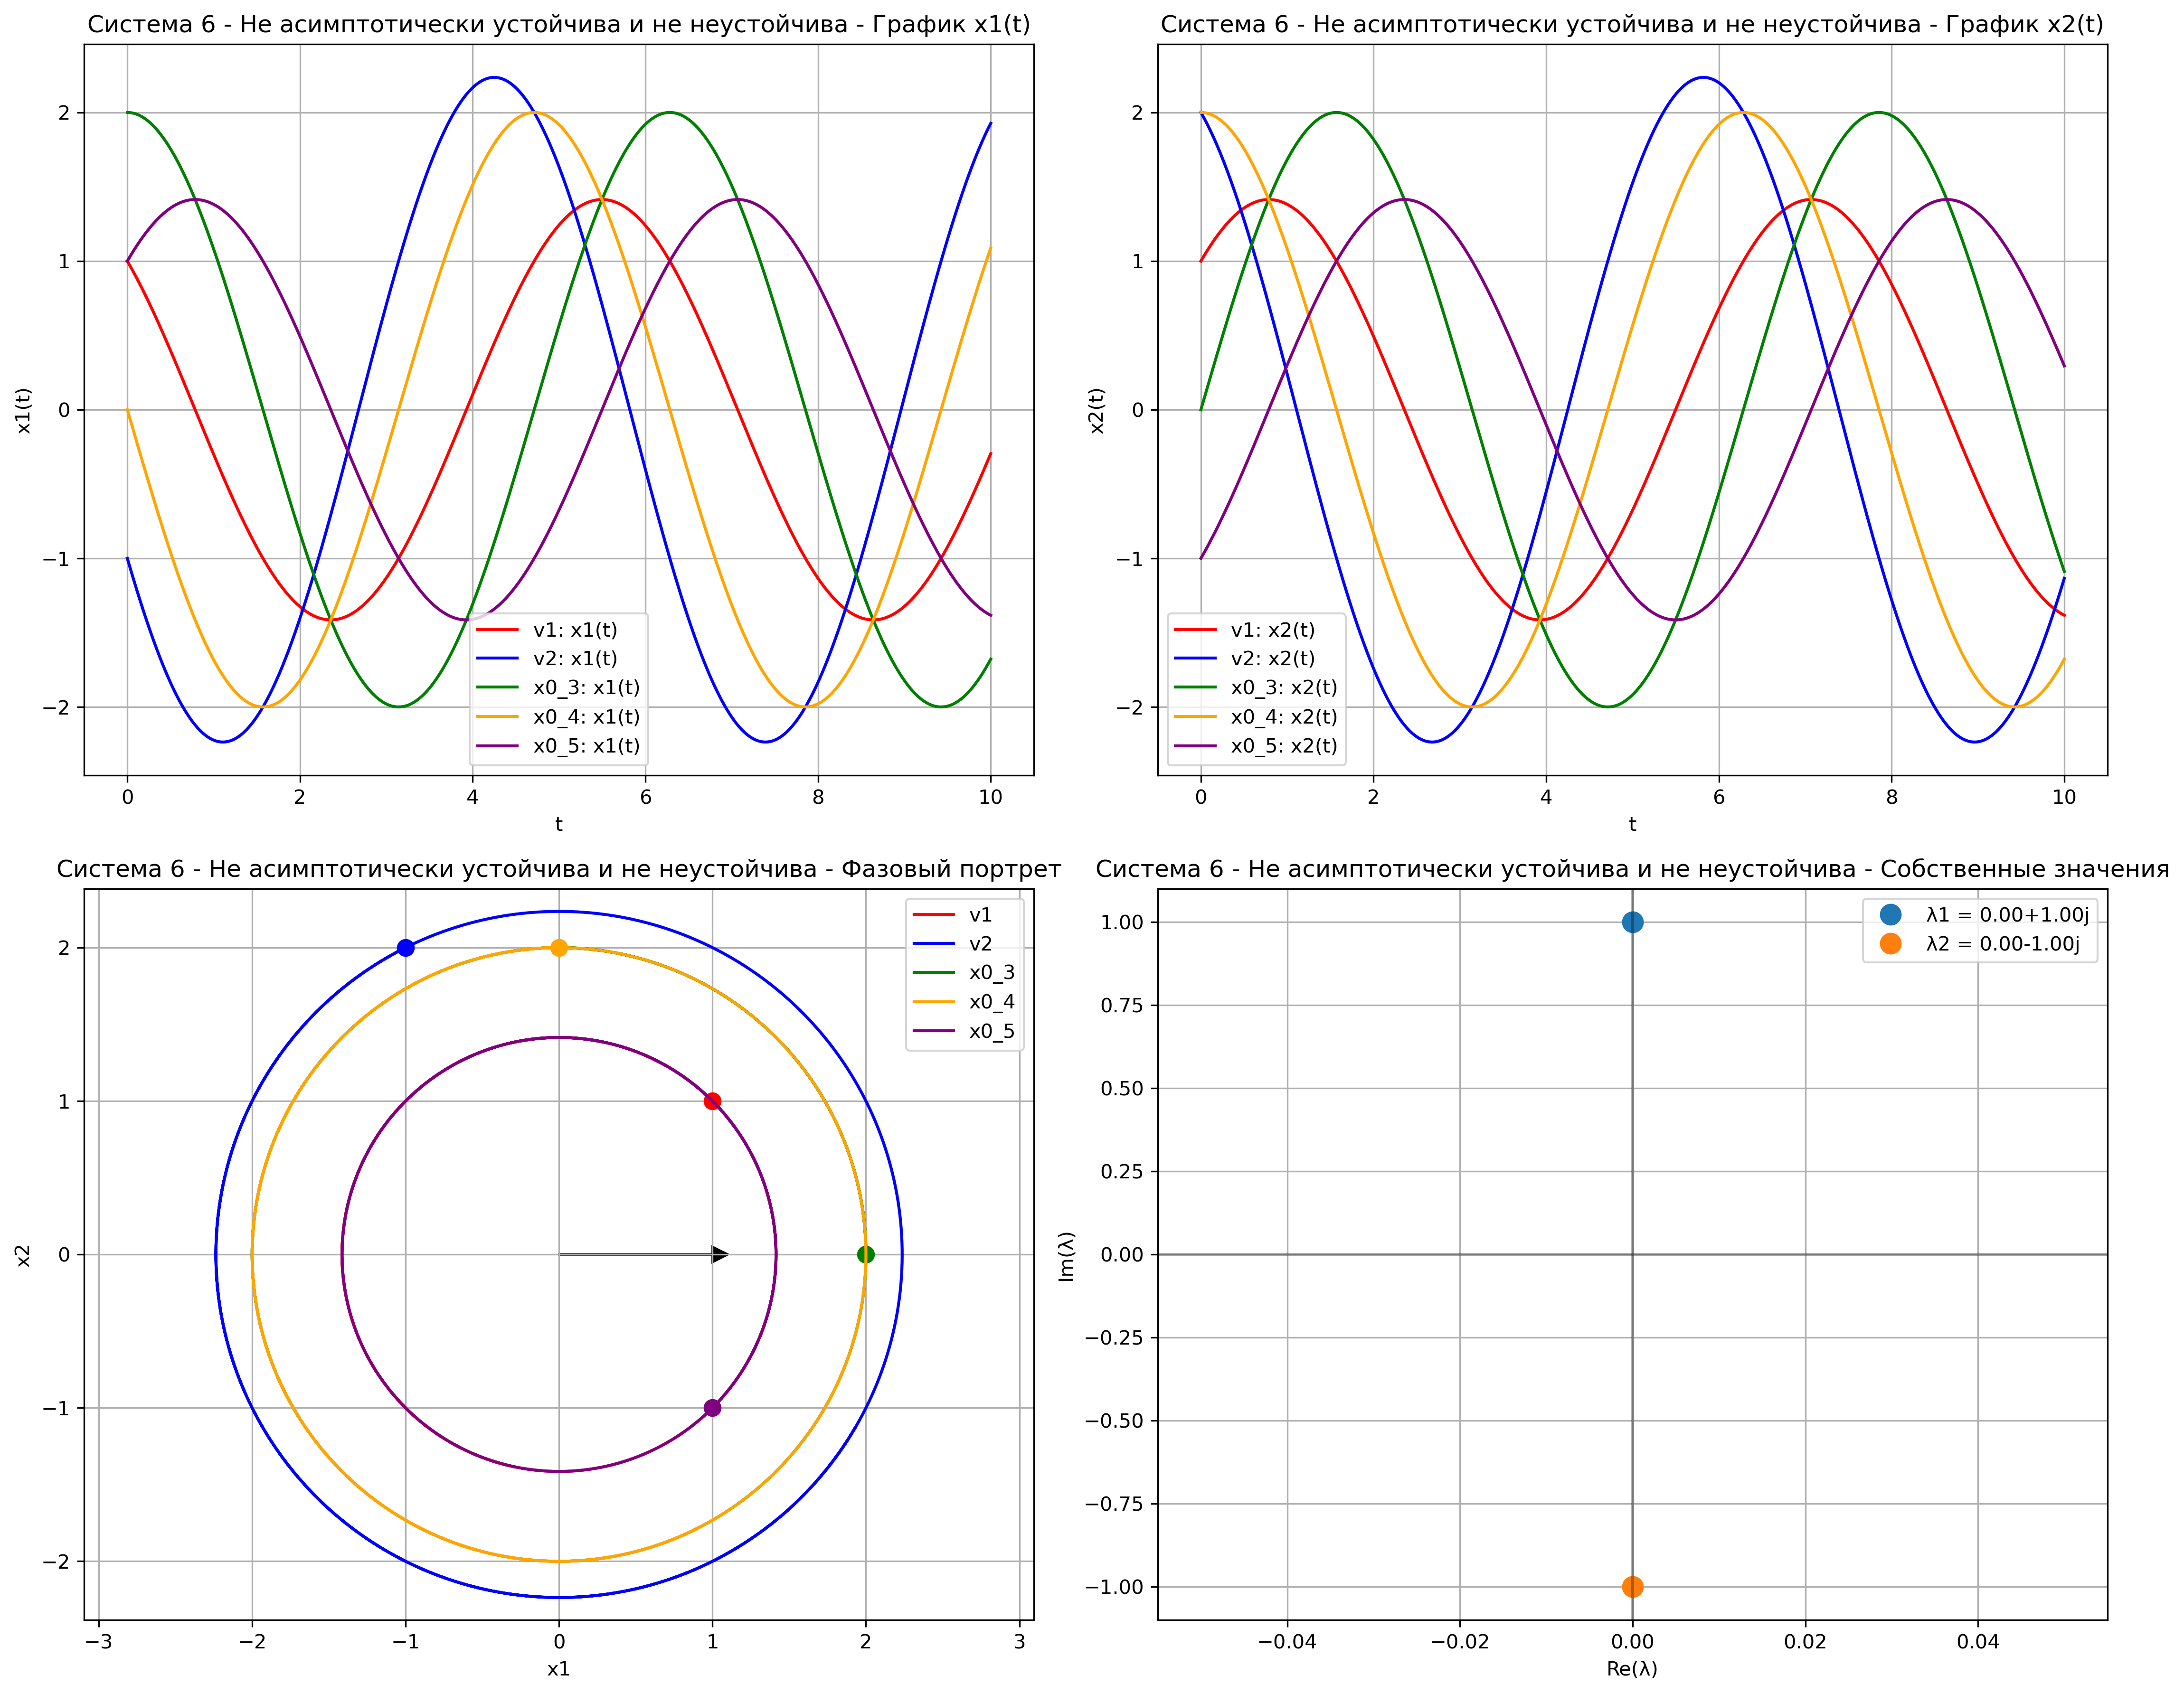
\includegraphics[width=0.8\textwidth]{images/task1/система_6_-_не_асимптотически_устойчива_и_не_неустойчива.png}
\caption{Система 6: Нейтрально устойчивая система}
\label{fig:system6}
\end{figure}

\section{Задание 2. Дискретные динамические системы}

В данном задании мы исследуем дискретные динамические системы второго порядка вида:
\begin{equation}
x(k+1) = Ax(k), \quad x(k) \in \mathbb{R}^2, \quad A \in \mathbb{R}^{2 \times 2}
\end{equation}

\subsection{Создание матриц с заданными собственными значениями}

Для создания матриц с заданными собственными значениями используем формулу:
\begin{equation}
A = P \cdot D \cdot P^{-1}
\end{equation}
где $D$ - диагональная матрица с собственными значениями, а $P$ - недиагональная матрица перехода.

\subsection{Системы с различными собственными значениями}

1. $\lambda_{1,2} = -1$ - система с отрицательными собственными значениями
2. $\lambda_{1,2} = -\frac{1}{\sqrt{2}} \pm \frac{1}{\sqrt{2}}i$ - система с комплексными собственными значениями внутри единичного круга
3. $\lambda_{1,2} = \pm i$ - система с мнимыми собственными значениями на единичной окружности
4. $\lambda_{1,2} = \frac{1}{\sqrt{2}} \pm \frac{1}{\sqrt{2}}i$ - система с комплексными собственными значениями внутри единичного круга
5. $\lambda_{1,2} = 1$ - система с единичными собственными значениями

6-8. Те же собственные числа, умноженные на $c = 0.5$ ($0 < c < 1$)
9-11. Те же собственные числа, умноженные на $d = 1.5$ ($d > 1$)
12. $\lambda_{1,2} = 0$ - система с нулевыми собственными значениями

\subsection{Моделирование дискретных систем}

На рис. \ref{fig:discrete_systems} представлены графики для всех двенадцати систем.

\begin{figure}[h!]
\centering
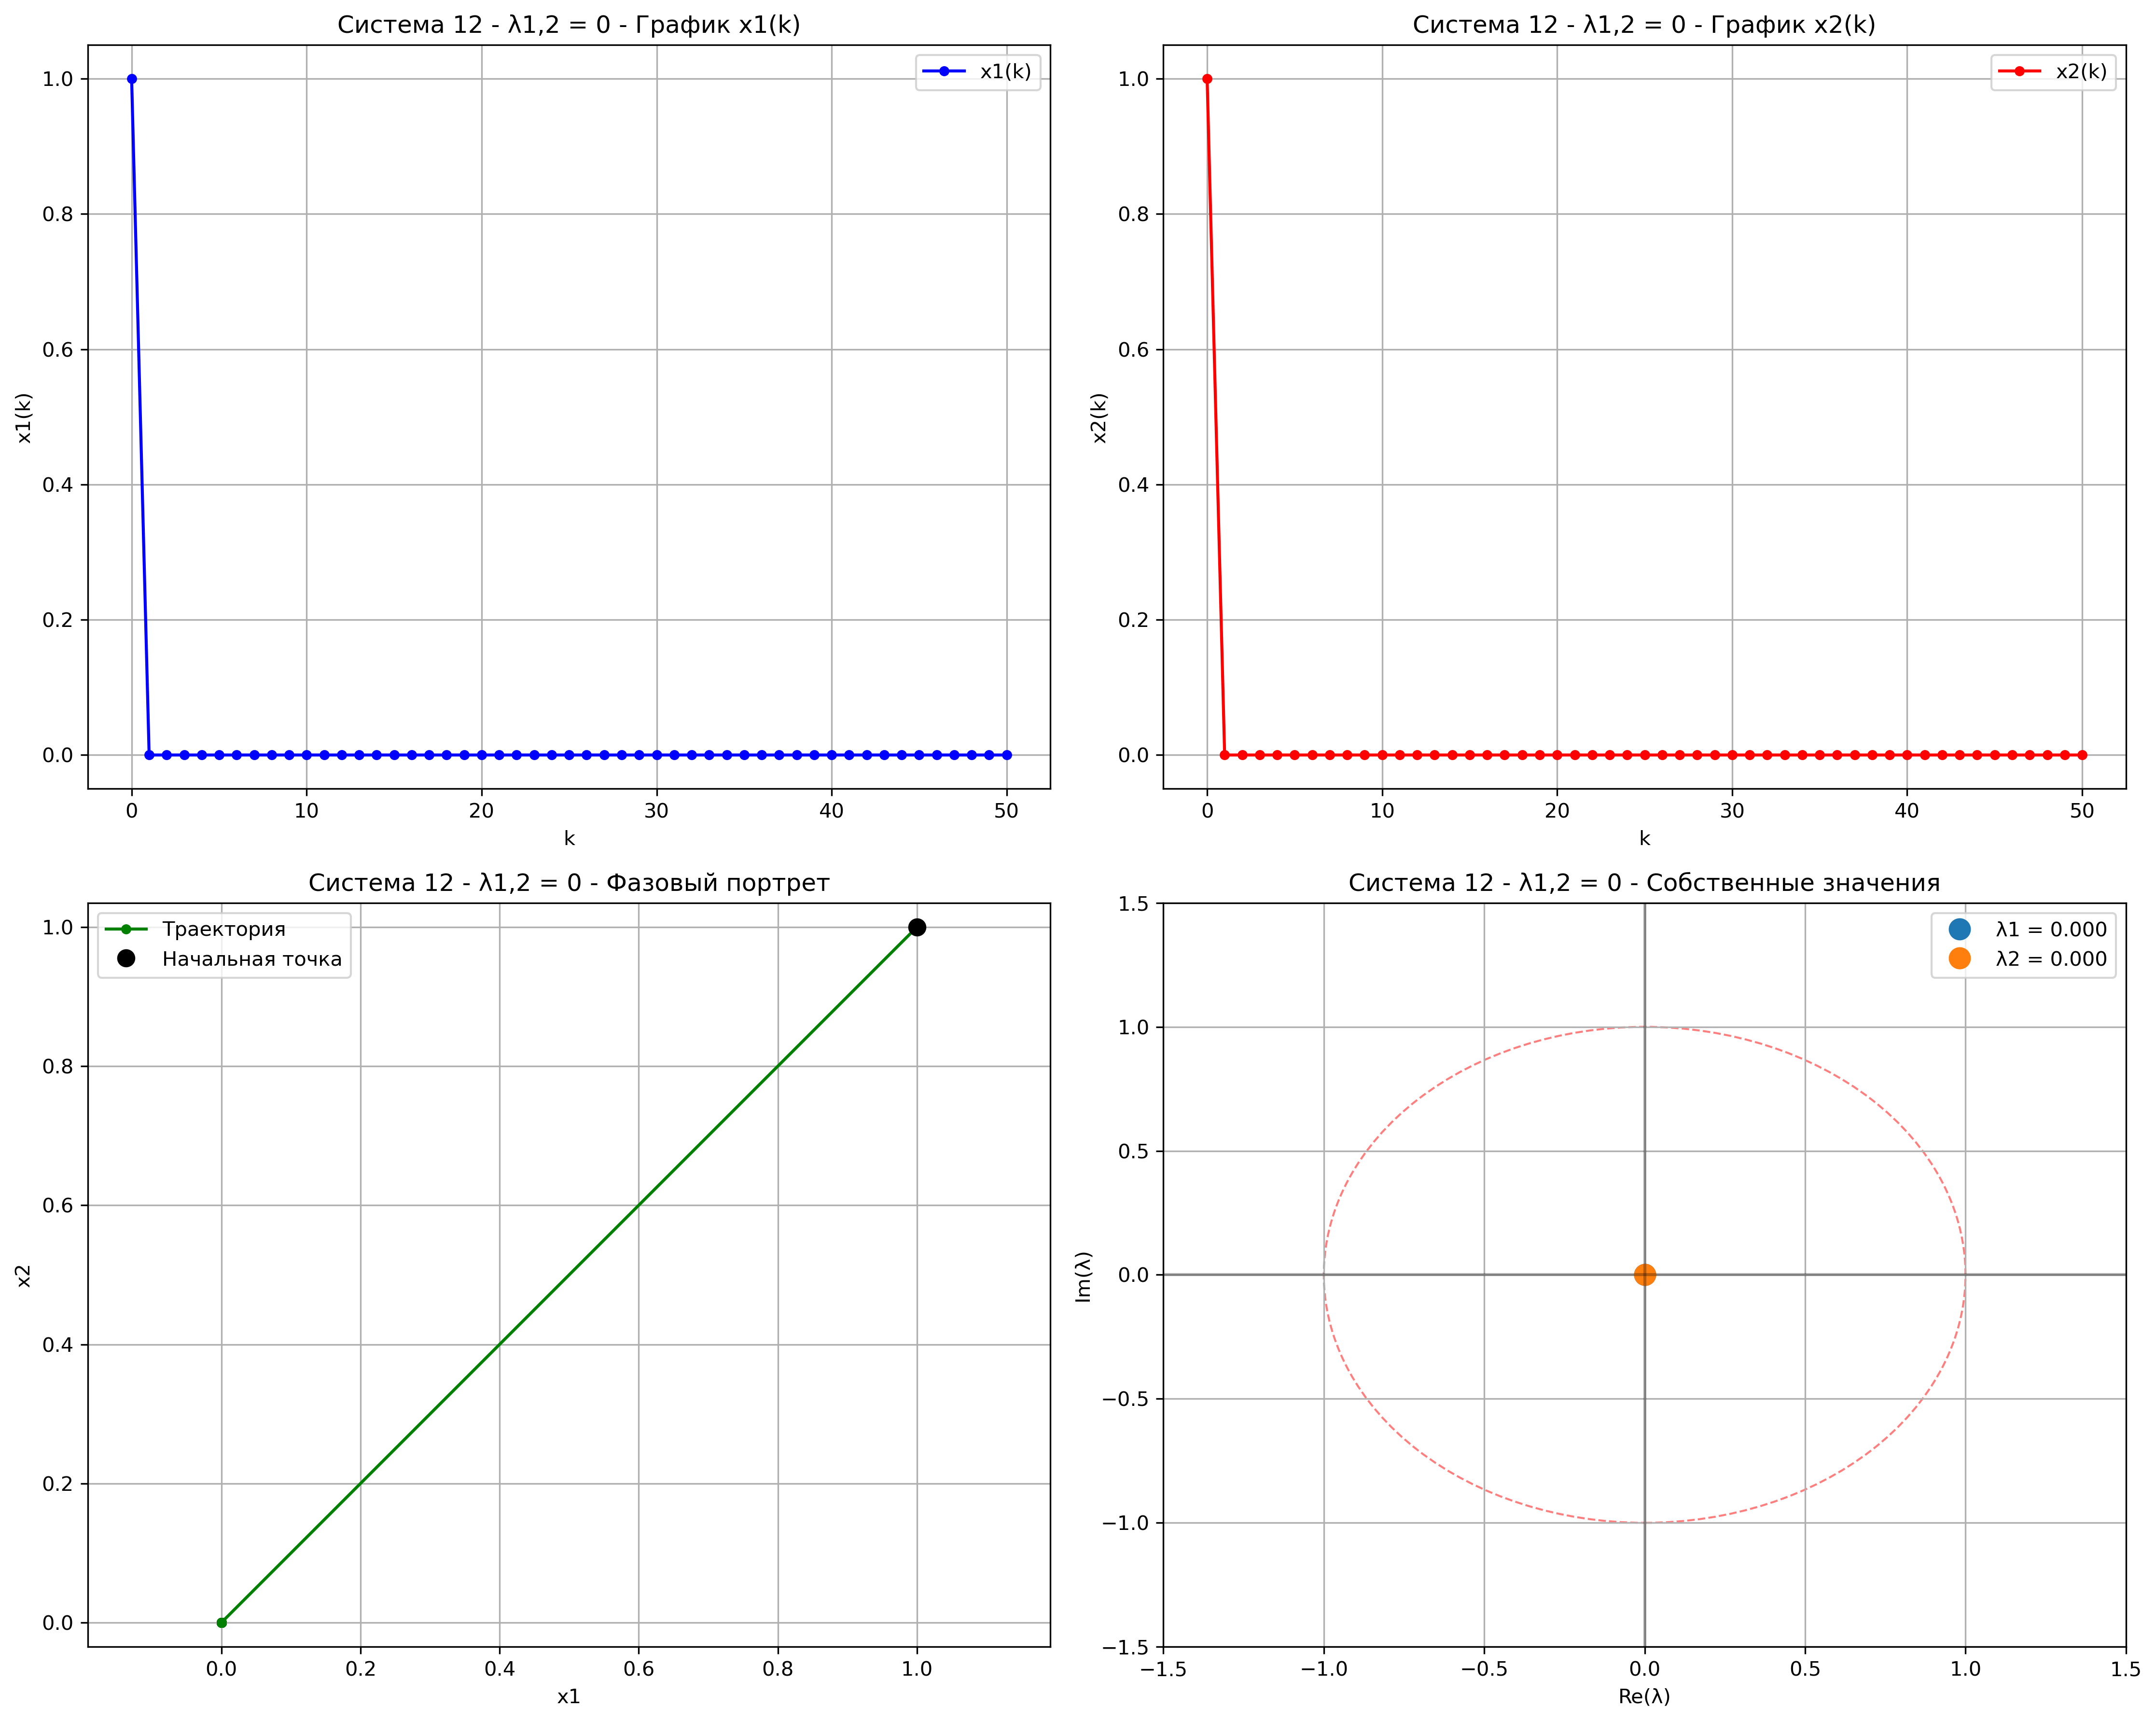
\includegraphics[width=0.8\textwidth]{images/task2/system_1_lambda_minus_1.png}
\caption{Система 1: $\lambda_{1,2} = -1$}
\label{fig:discrete1}
\end{figure}

\begin{figure}[h!]
\centering
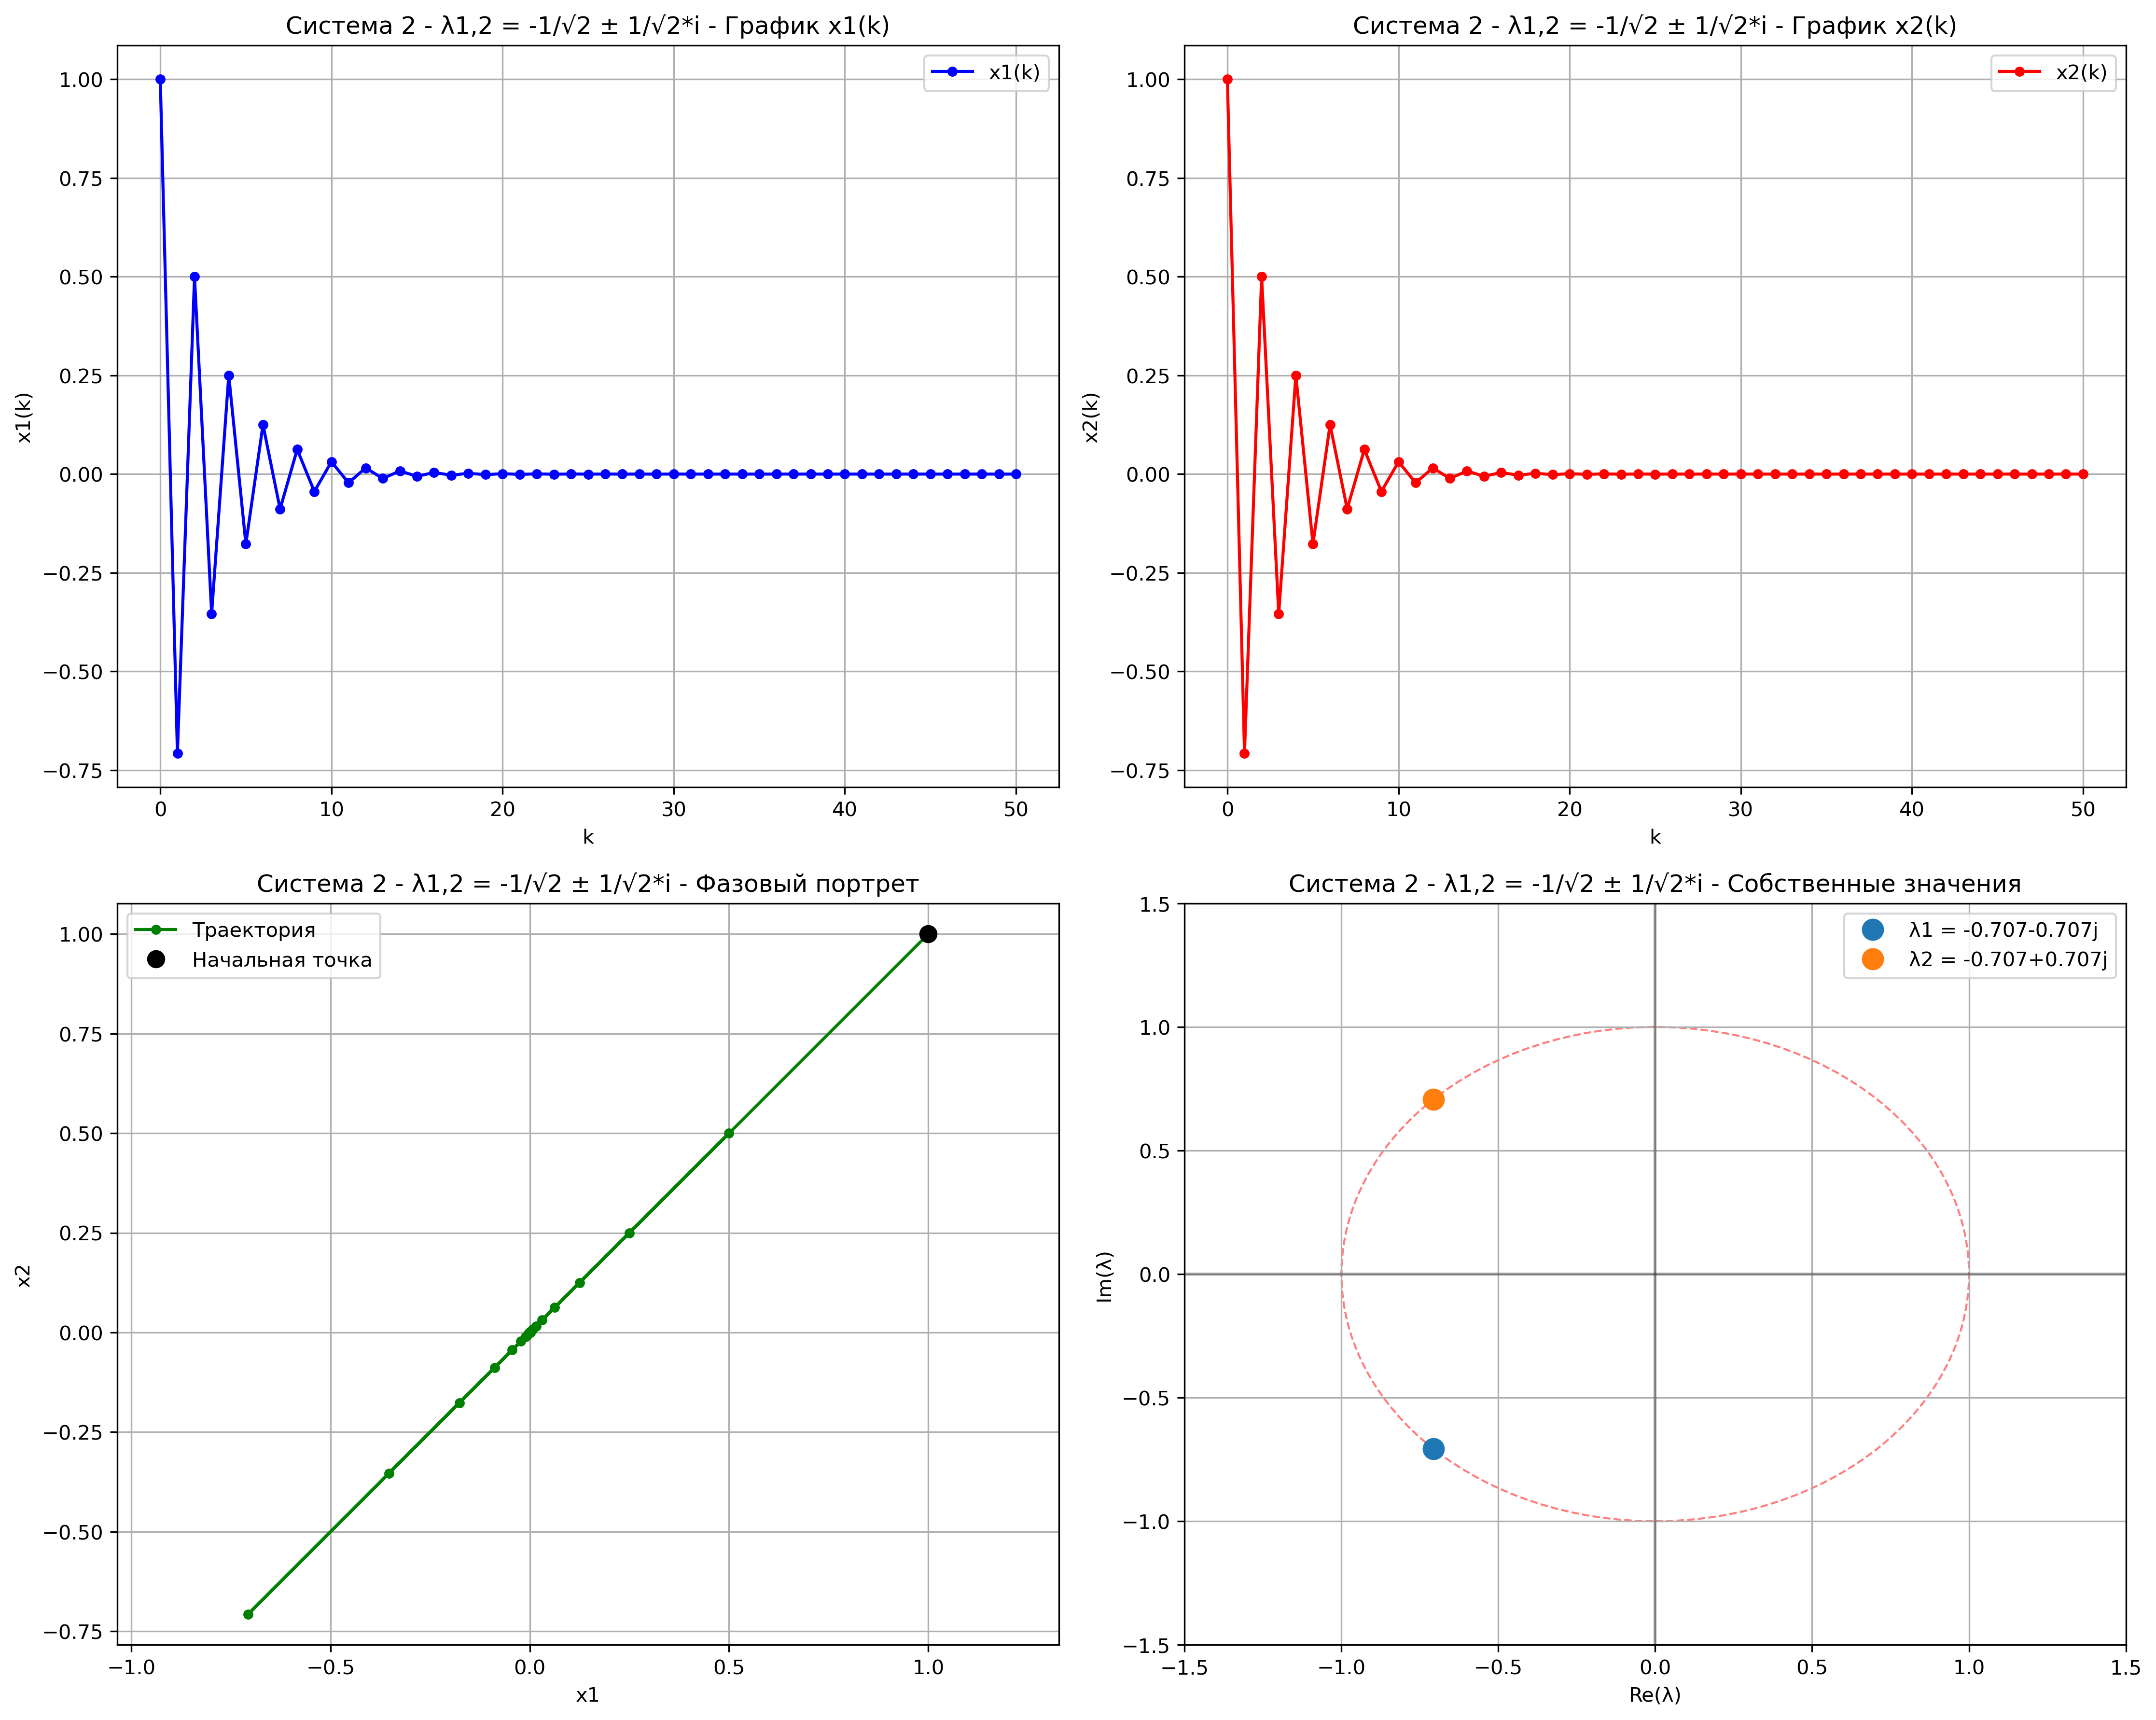
\includegraphics[width=0.8\textwidth]{images/task2/system_2_lambda_minus_1_sqrt2_pm_i_sqrt2.png}
\caption{Система 2: $\lambda_{1,2} = -\frac{1}{\sqrt{2}} \pm \frac{1}{\sqrt{2}}i$}
\label{fig:discrete2}
\end{figure}

\begin{figure}[h!]
\centering
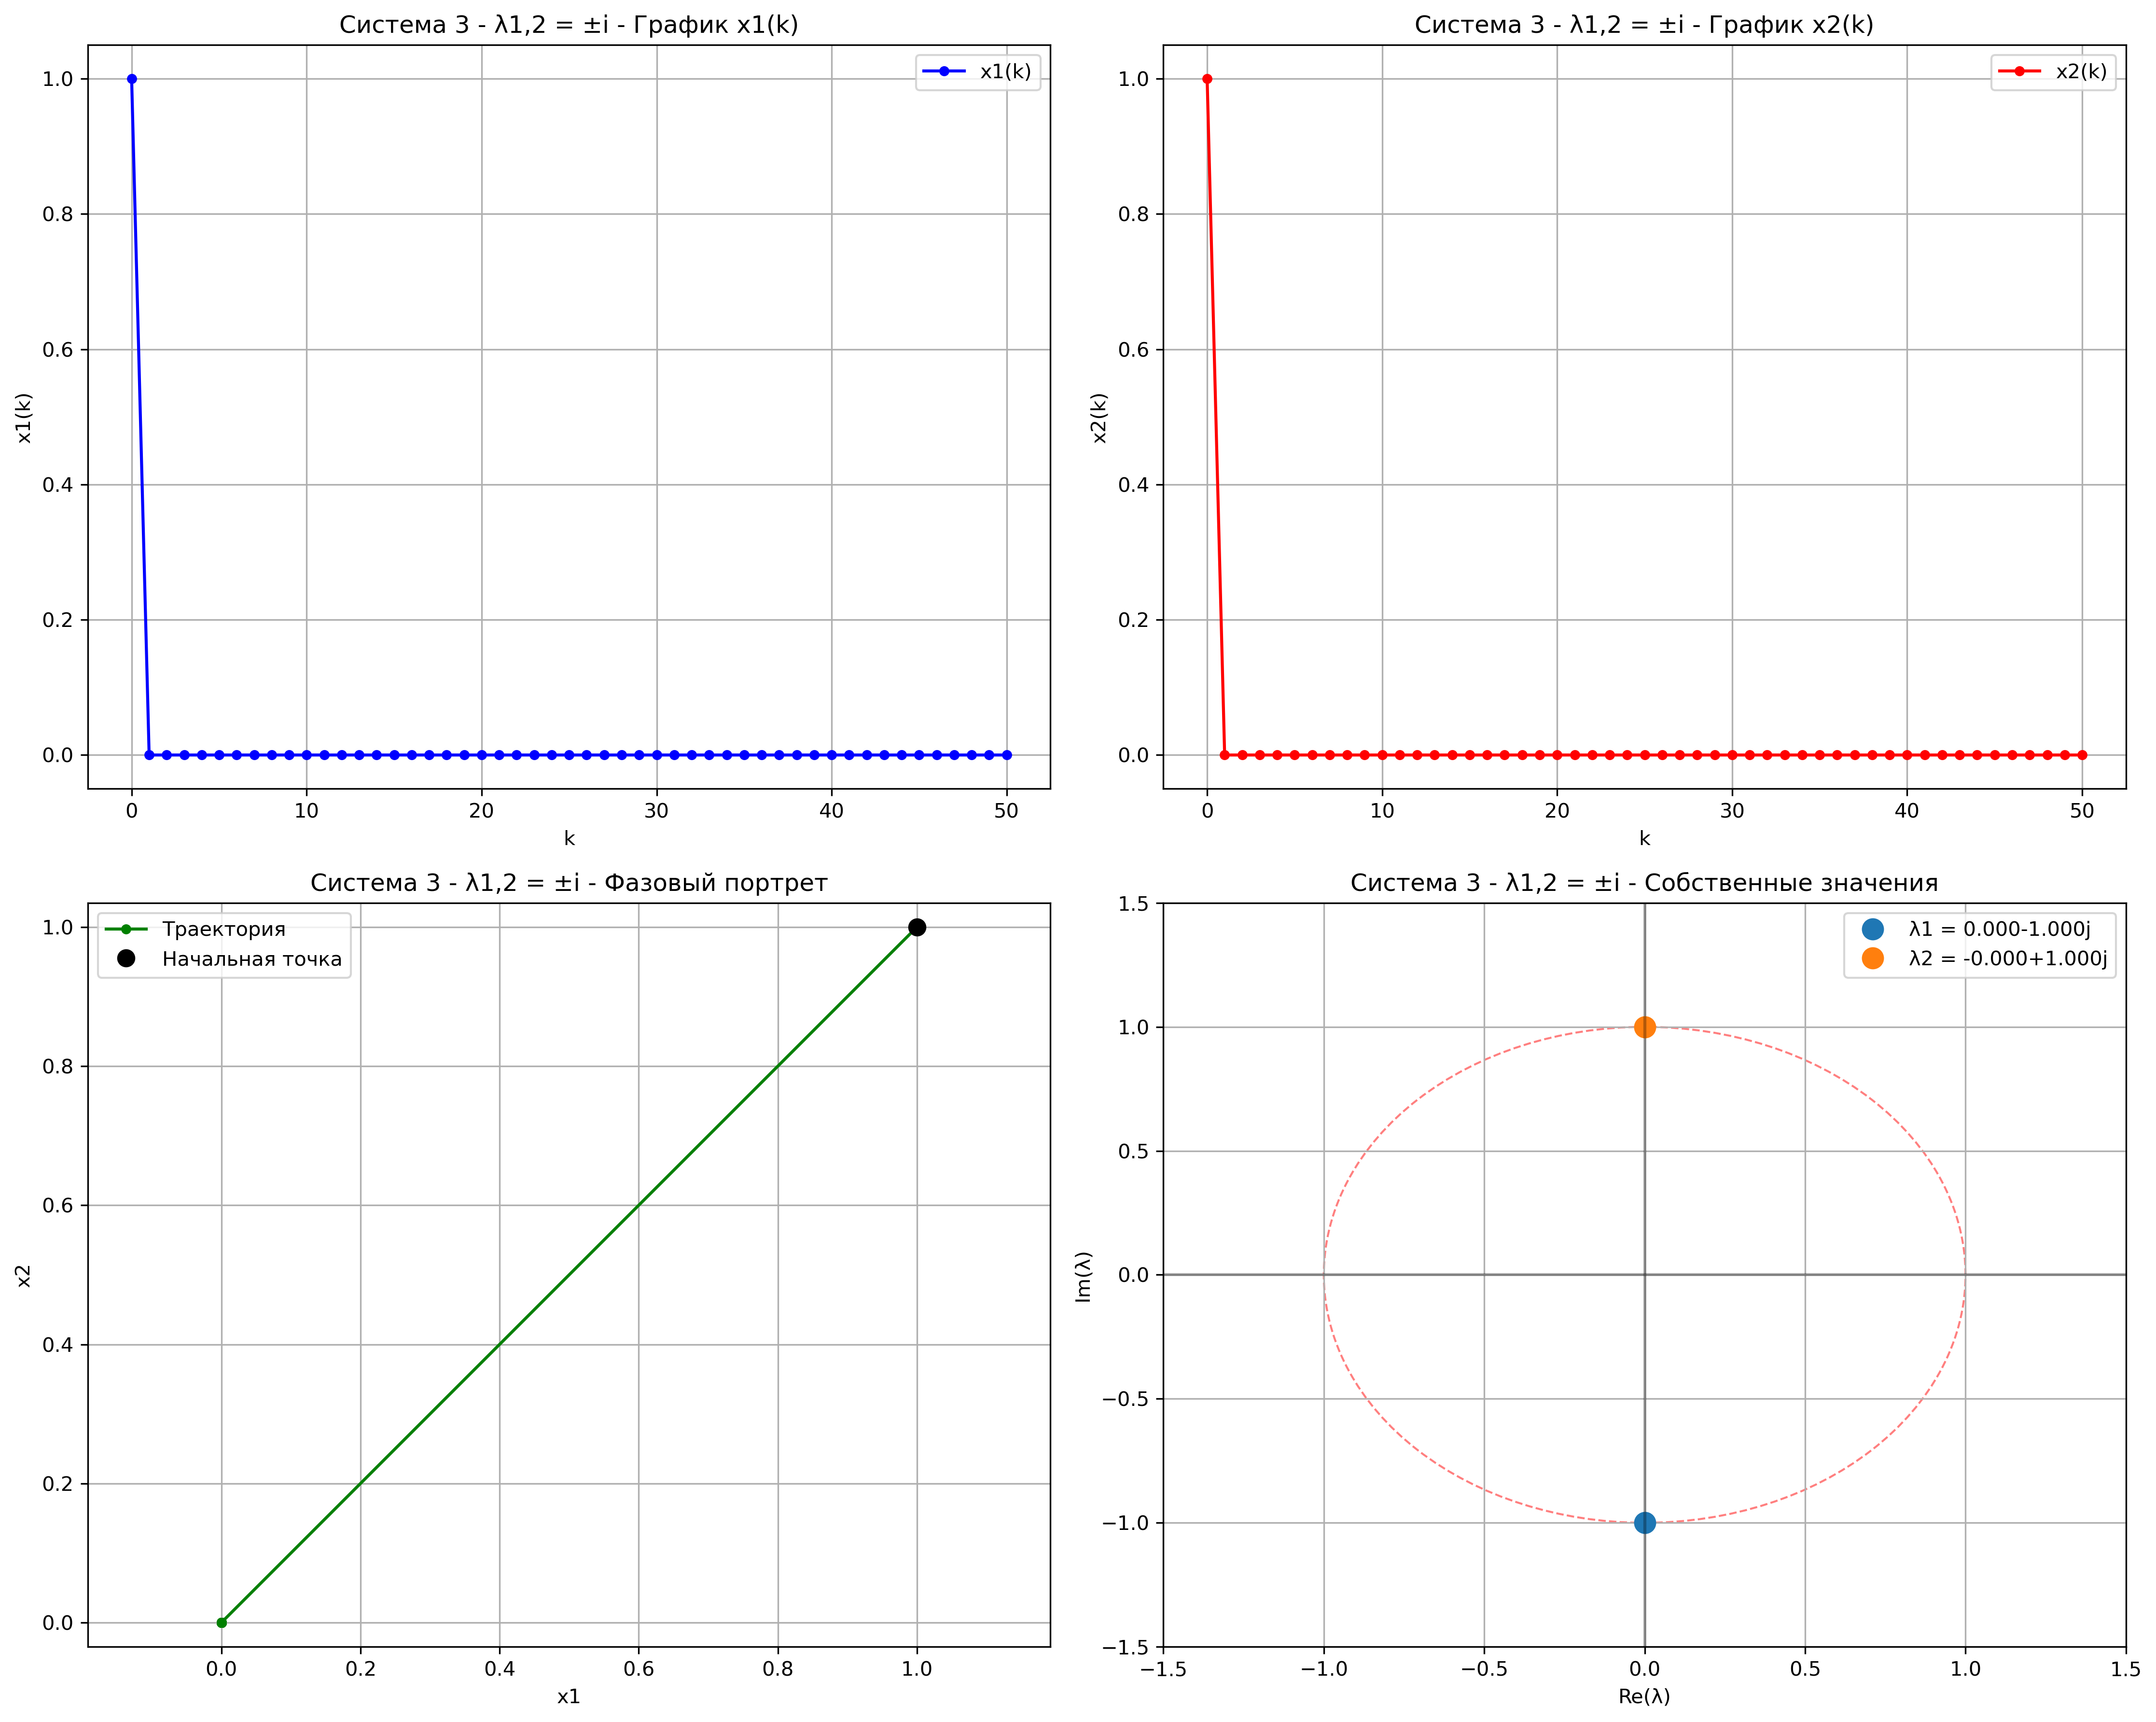
\includegraphics[width=0.8\textwidth]{images/task2/system_3_lambda_pm_i.png}
\caption{Система 3: $\lambda_{1,2} = \pm i$}
\label{fig:discrete3}
\end{figure}

\begin{figure}[h!]
\centering
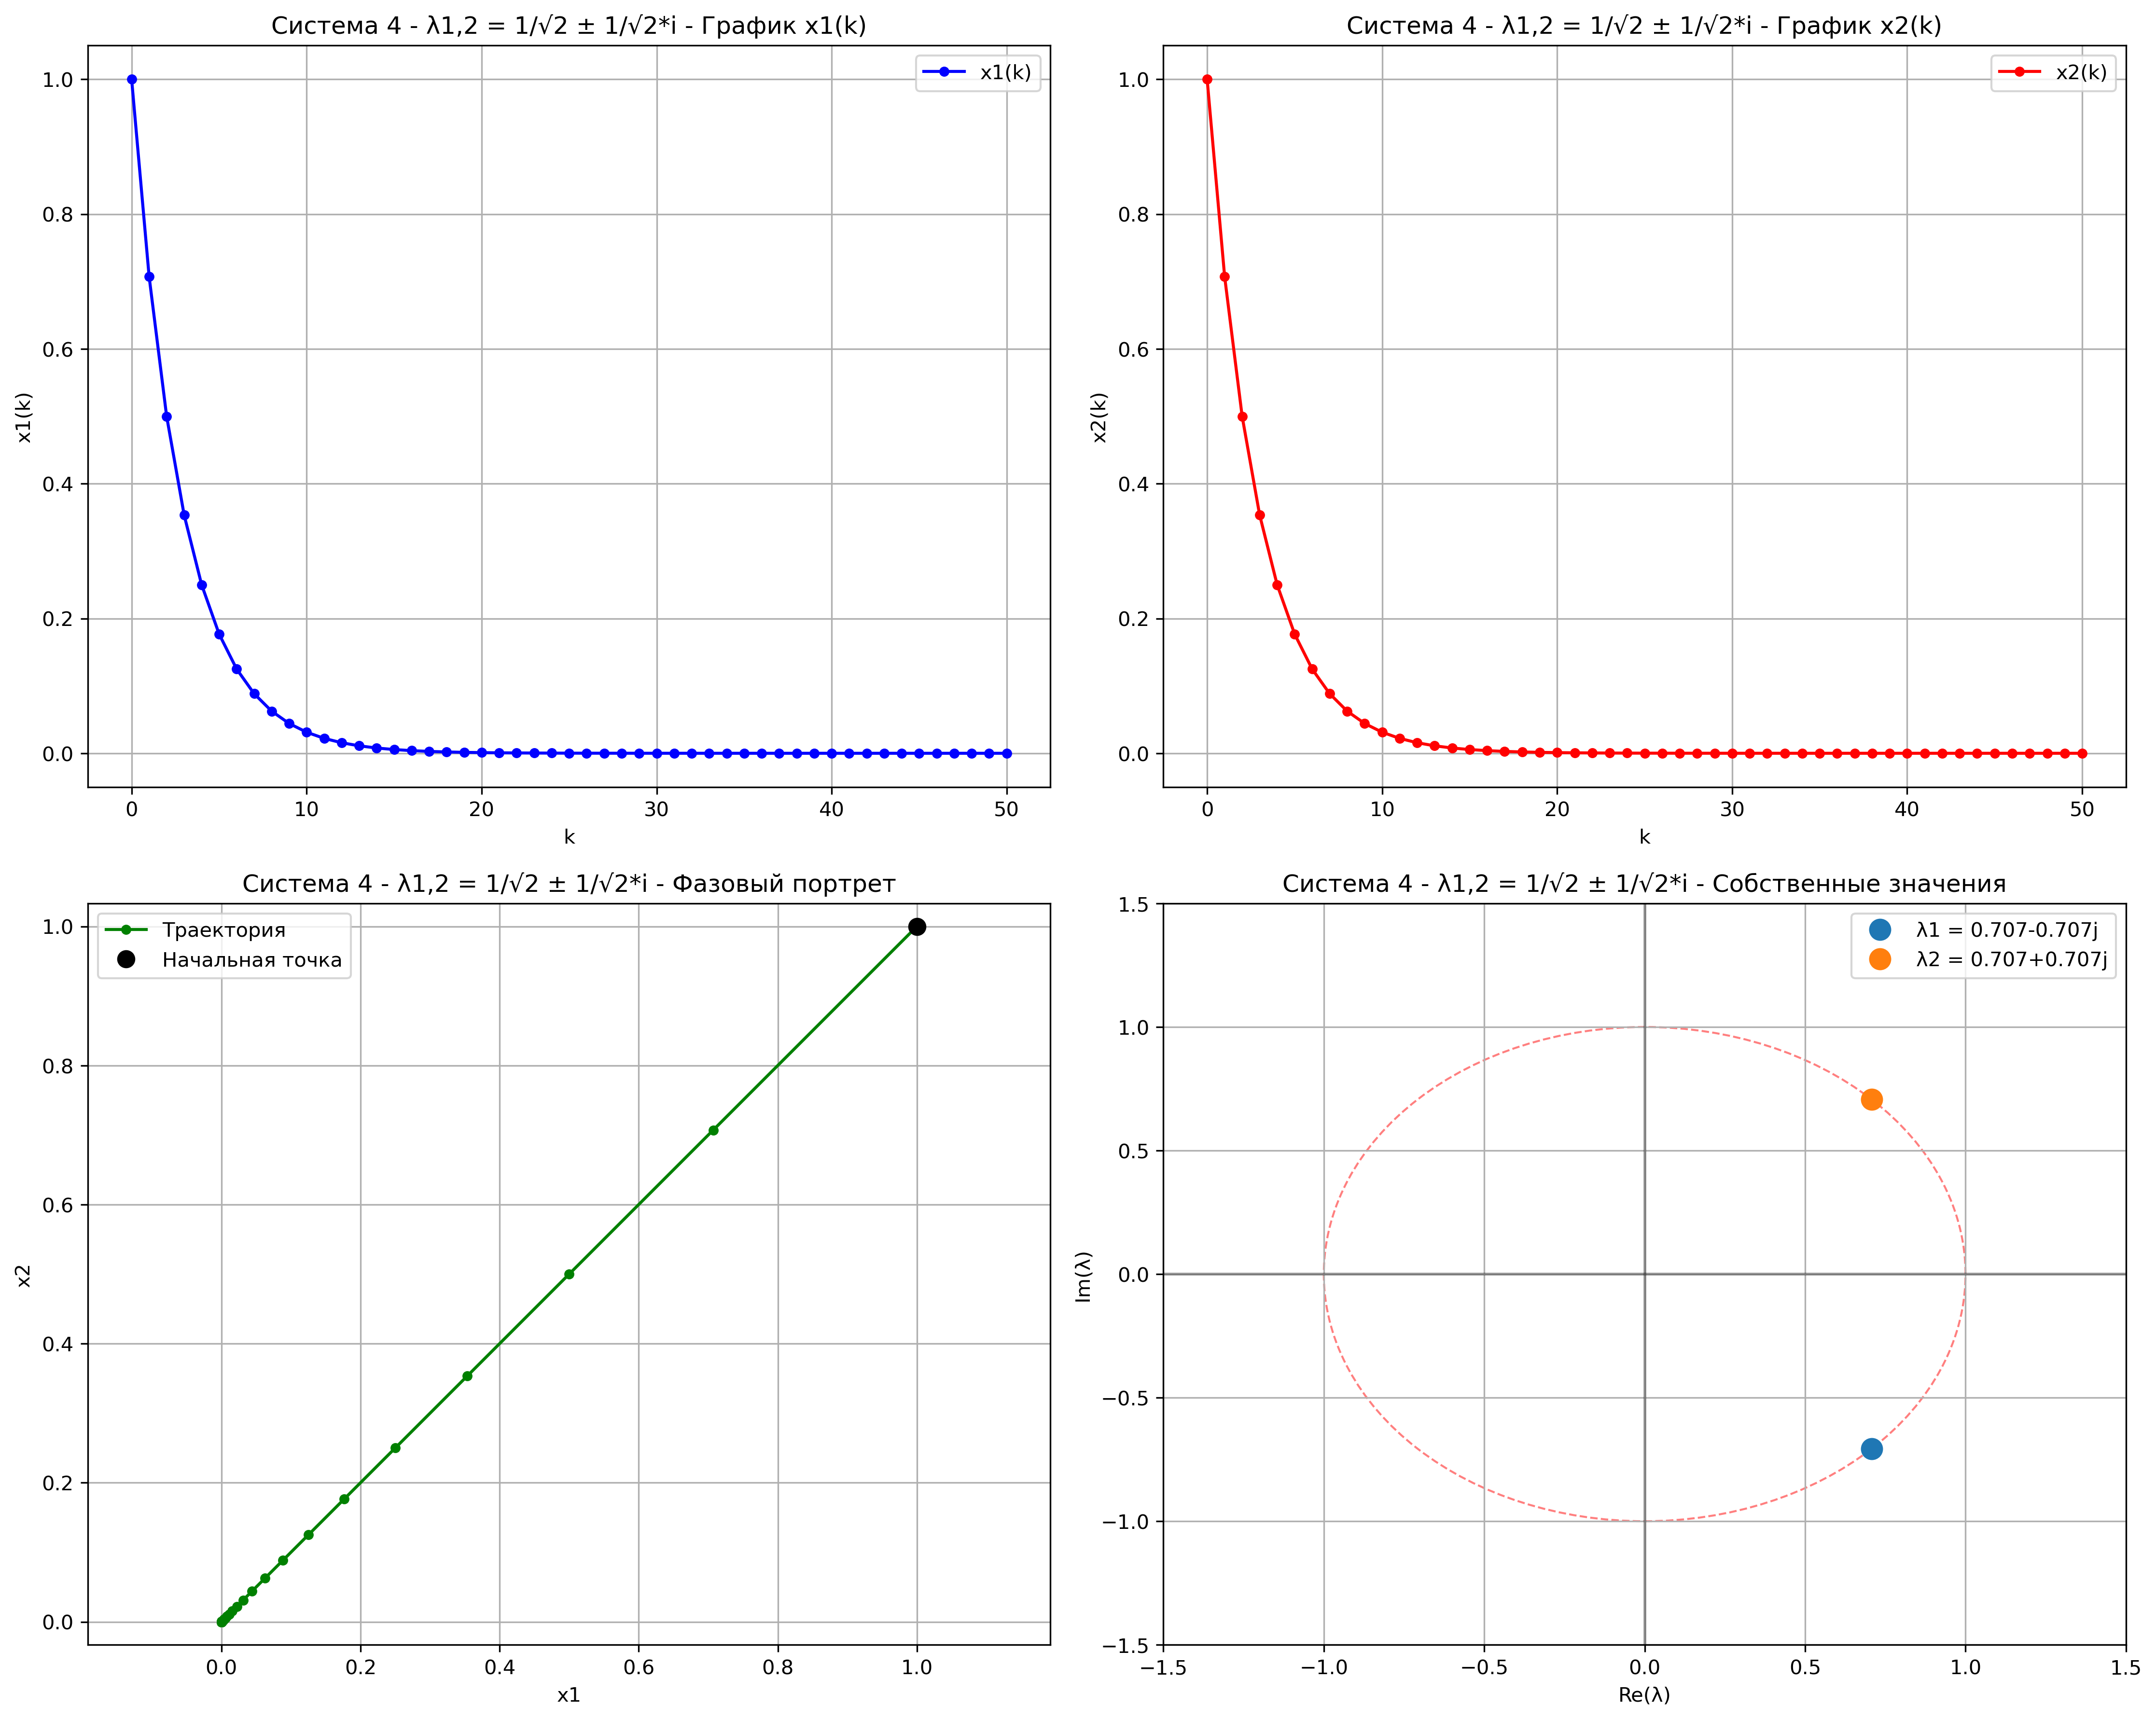
\includegraphics[width=0.8\textwidth]{images/task2/system_4_lambda_1_sqrt2_pm_i_sqrt2.png}
\caption{Система 4: $\lambda_{1,2} = \frac{1}{\sqrt{2}} \pm \frac{1}{\sqrt{2}}i$}
\label{fig:discrete4}
\end{figure}

\begin{figure}[h!]
\centering
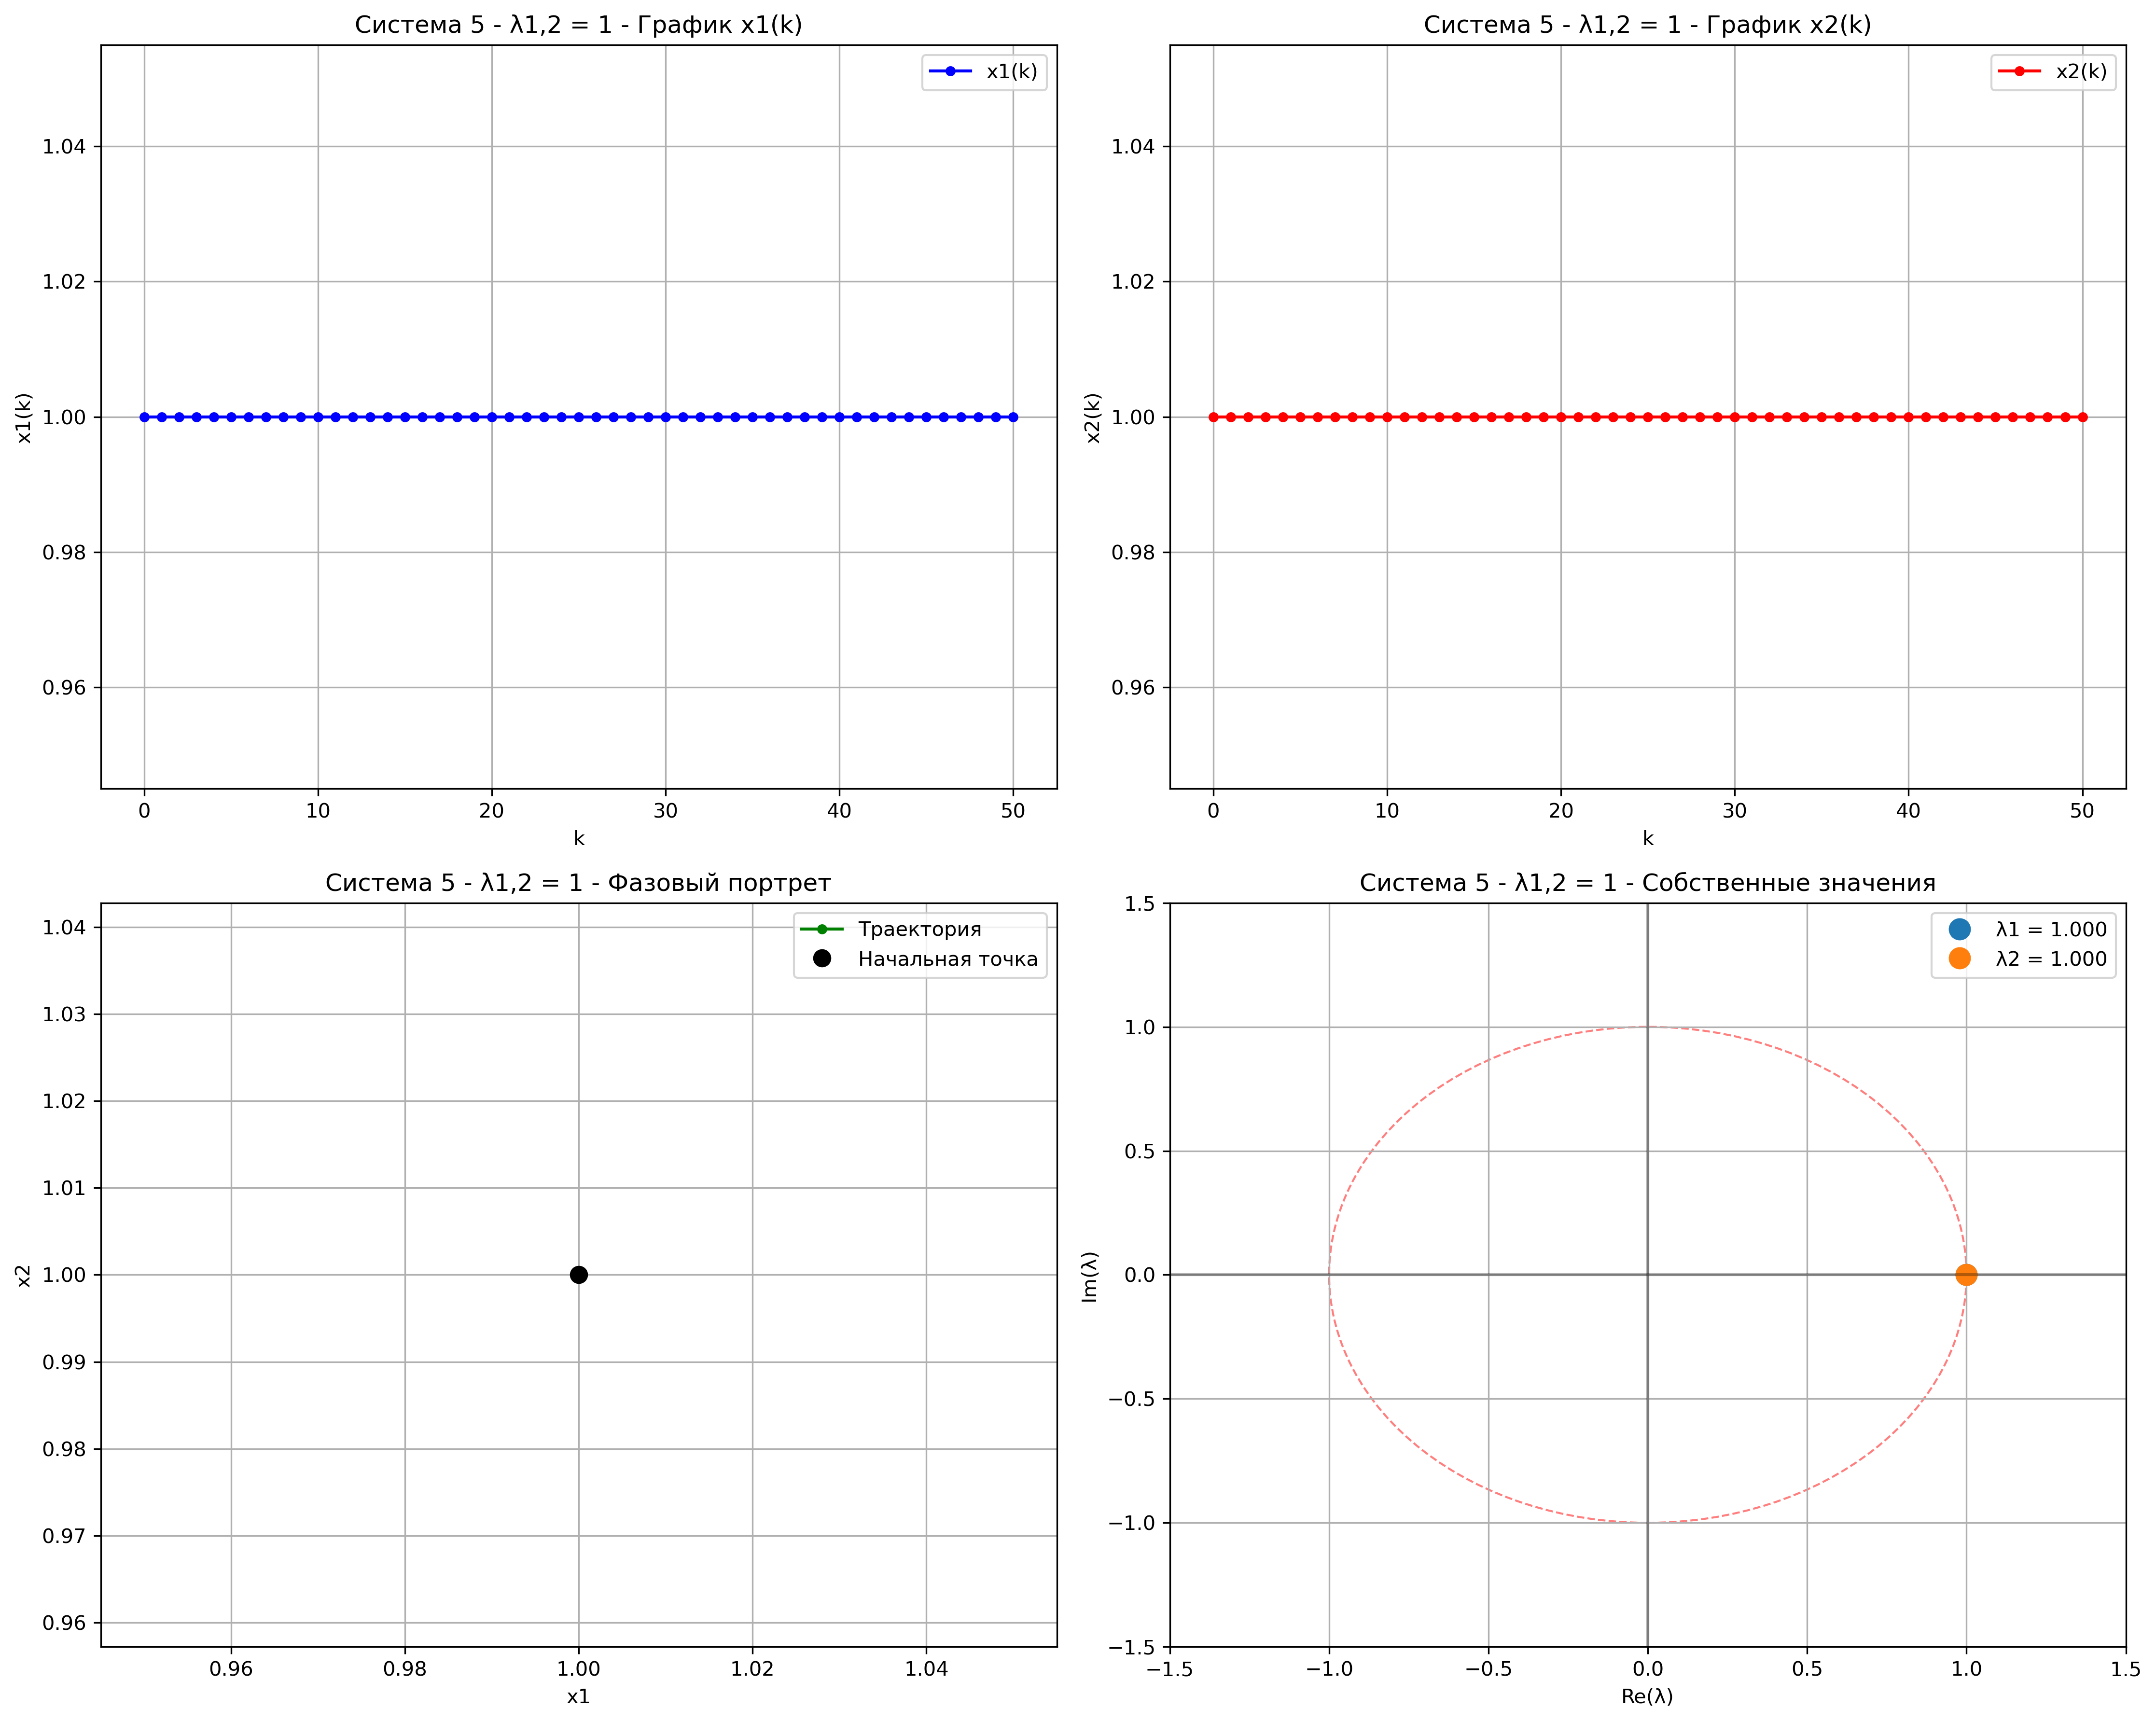
\includegraphics[width=0.8\textwidth]{images/task2/system_5_lambda_1.png}
\caption{Система 5: $\lambda_{1,2} = 1$}
\label{fig:discrete5}
\end{figure}

\section{Задание 3. Осциллятор}

Рассмотрим непрерывную систему вида:
\begin{equation}
\begin{cases}
\dot{x}_1 = x_2 \\
\dot{x}_2 = ax_1 + bx_2
\end{cases}
\end{equation}

Матрица системы:
\begin{equation}
A = \begin{pmatrix} 0 & 1 \\ a & b \end{pmatrix}
\end{equation}

Характеристическое уравнение:
\begin{equation}
\det(A - \lambda I) = \begin{vmatrix} -\lambda & 1 \\ a & b-\lambda \end{vmatrix} = \lambda^2 - b\lambda - a = 0
\end{equation}

Собственные значения:
\begin{equation}
\lambda_{1,2} = \frac{b \pm \sqrt{b^2 + 4a}}{2}
\end{equation}

\subsection{Случай 1: $a < 0$, $b = 0$}

Физическая интерпретация: Гармонический осциллятор без затухания (например, маятник без трения).

$x_1$ - смещение от положения равновесия
$x_2$ - скорость
$a$ - коэффициент упругости (отрицательный)
$b$ - коэффициент затухания (равен нулю)

Собственные значения: $\lambda_{1,2} = \pm \sqrt{-a}i$

Система нейтрально устойчива.

\begin{figure}[h!]
\centering
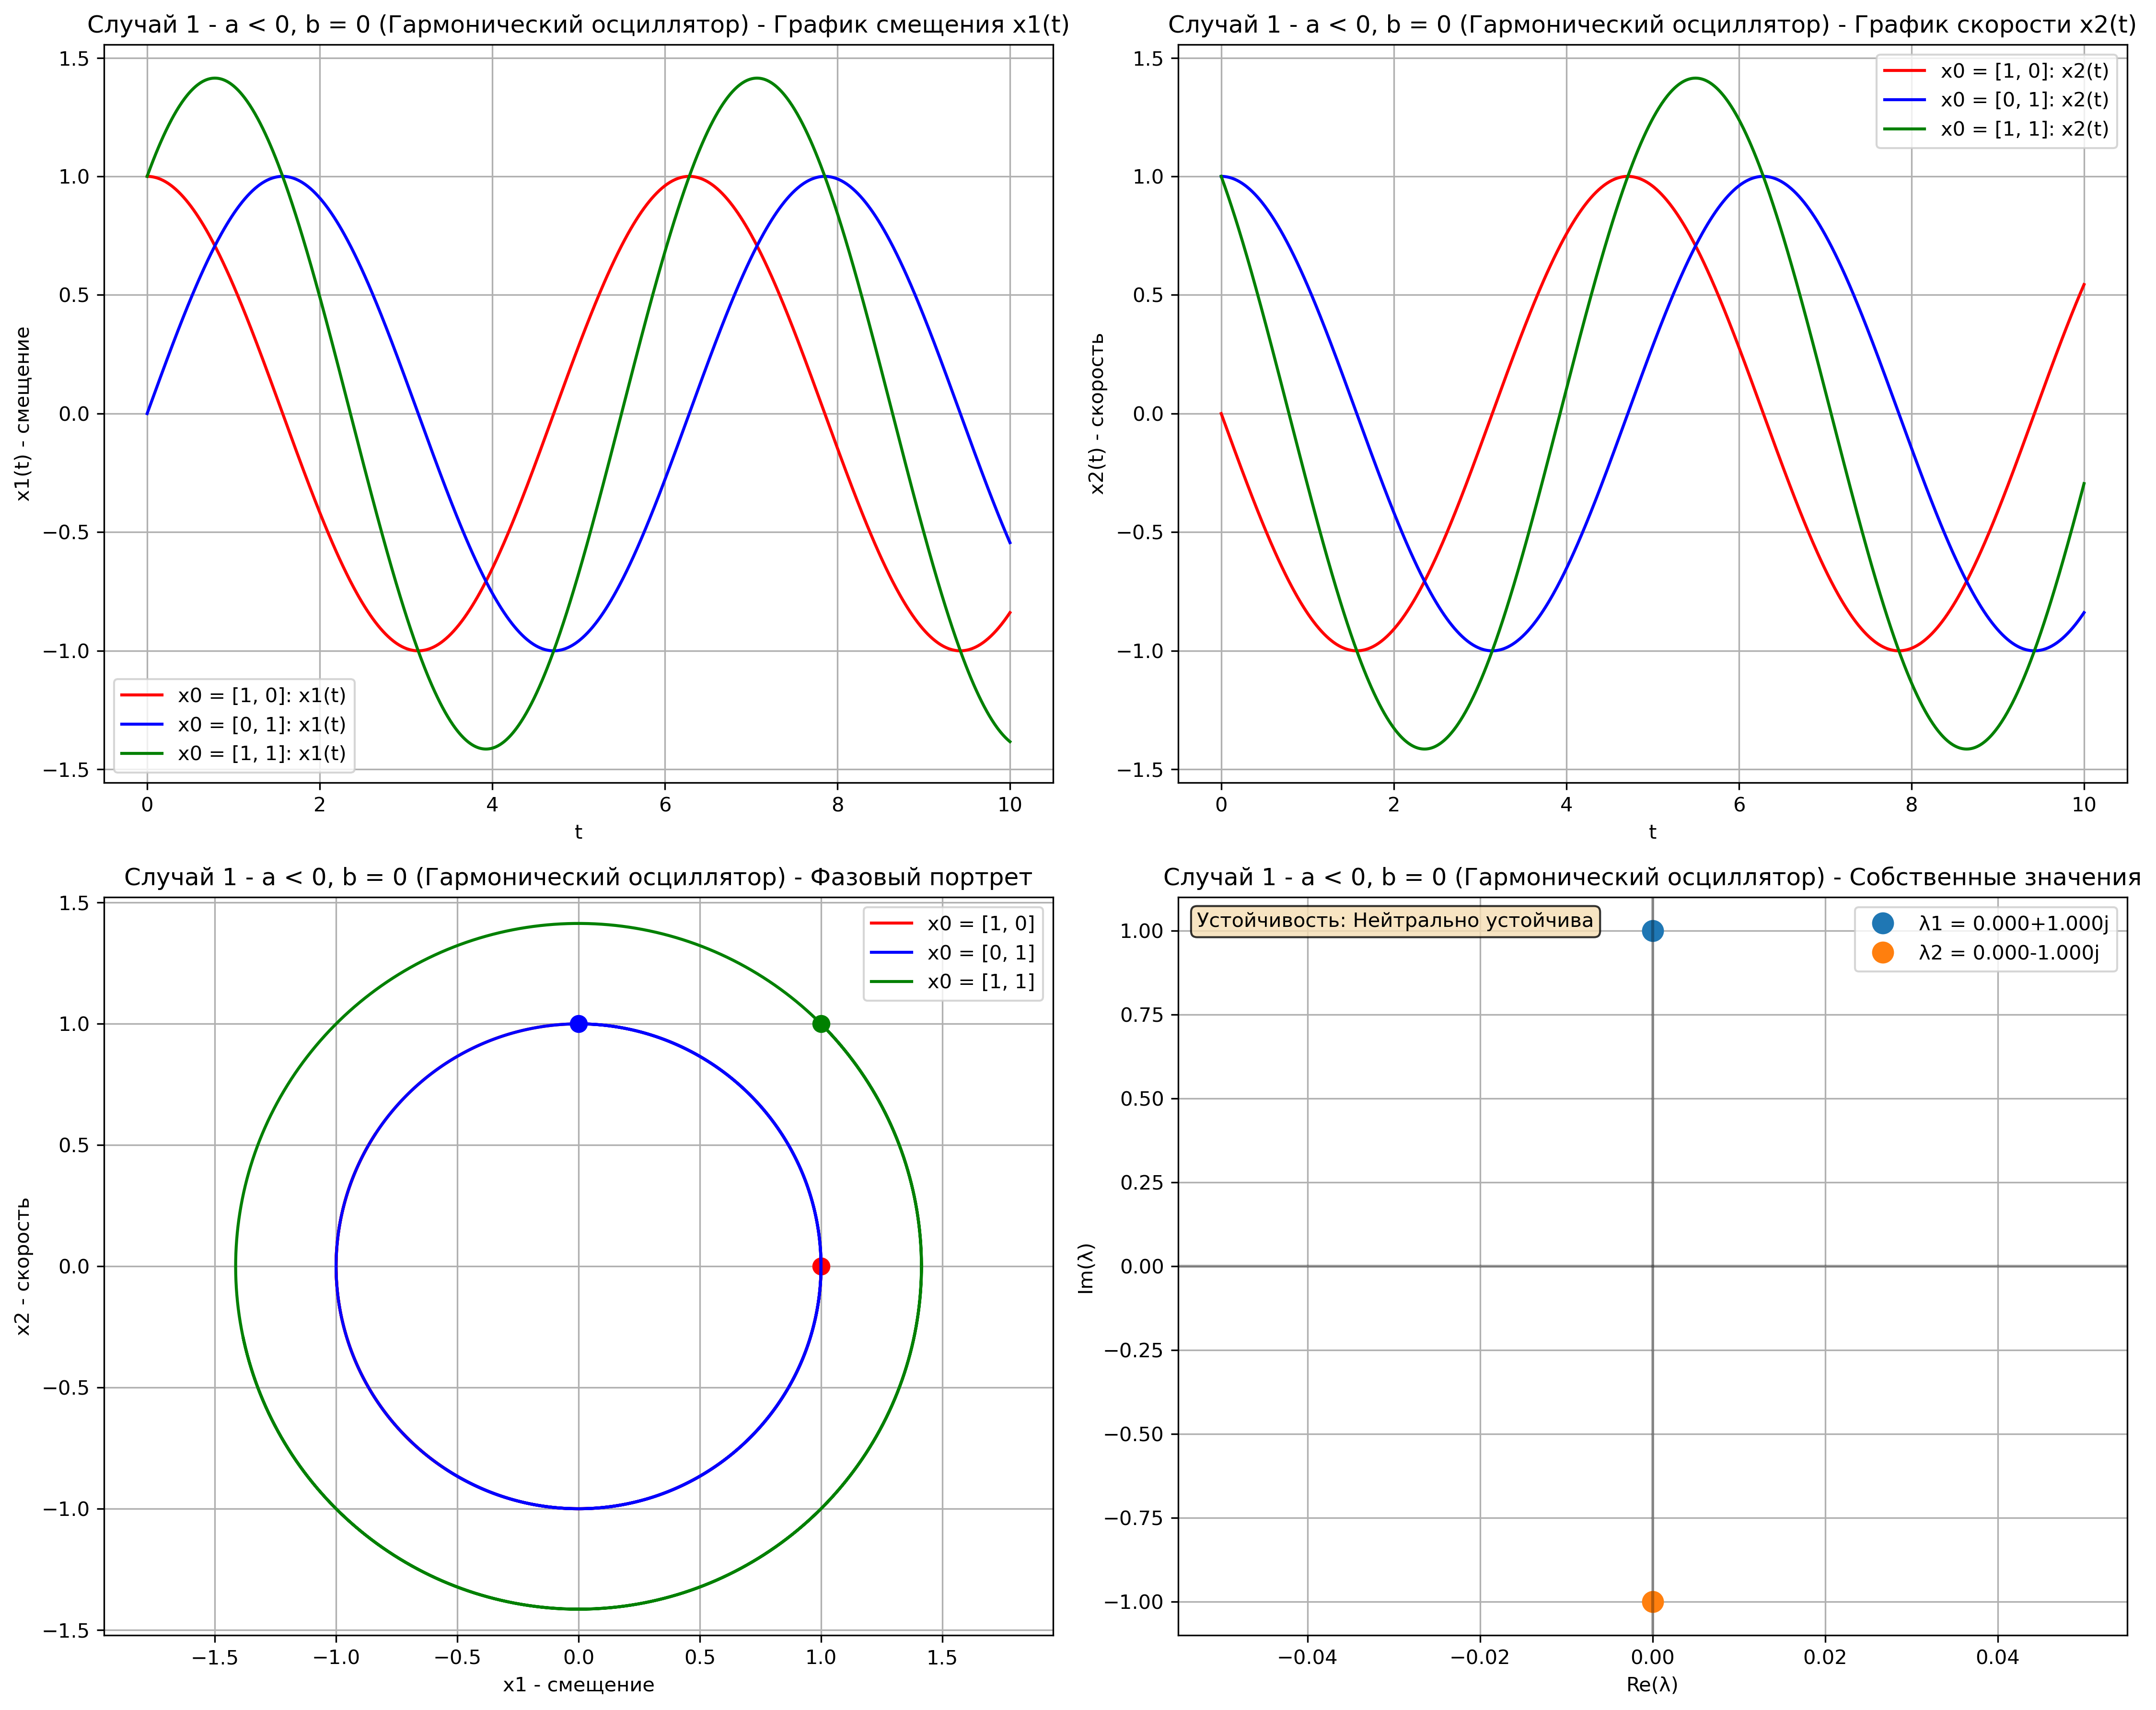
\includegraphics[width=0.8\textwidth]{images/task3/случай_1_-_a_<_0_b_=_0_гармонический_осциллятор.png}
\caption{Случай 1: Гармонический осциллятор без затухания}
\label{fig:oscillator1}
\end{figure}

\subsection{Случай 2: $a < 0$, $b < 0$}

Физическая интерпретация: Затухающий гармонический осциллятор (например, маятник с трением).

$x_1$ - смещение от положения равновесия
$x_2$ - скорость
$a$ - коэффициент упругости (отрицательный)
$b$ - коэффициент затухания (отрицательный)

Собственные значения имеют отрицательную вещественную часть.

Система асимптотически устойчива.

\begin{figure}[h!]
\centering
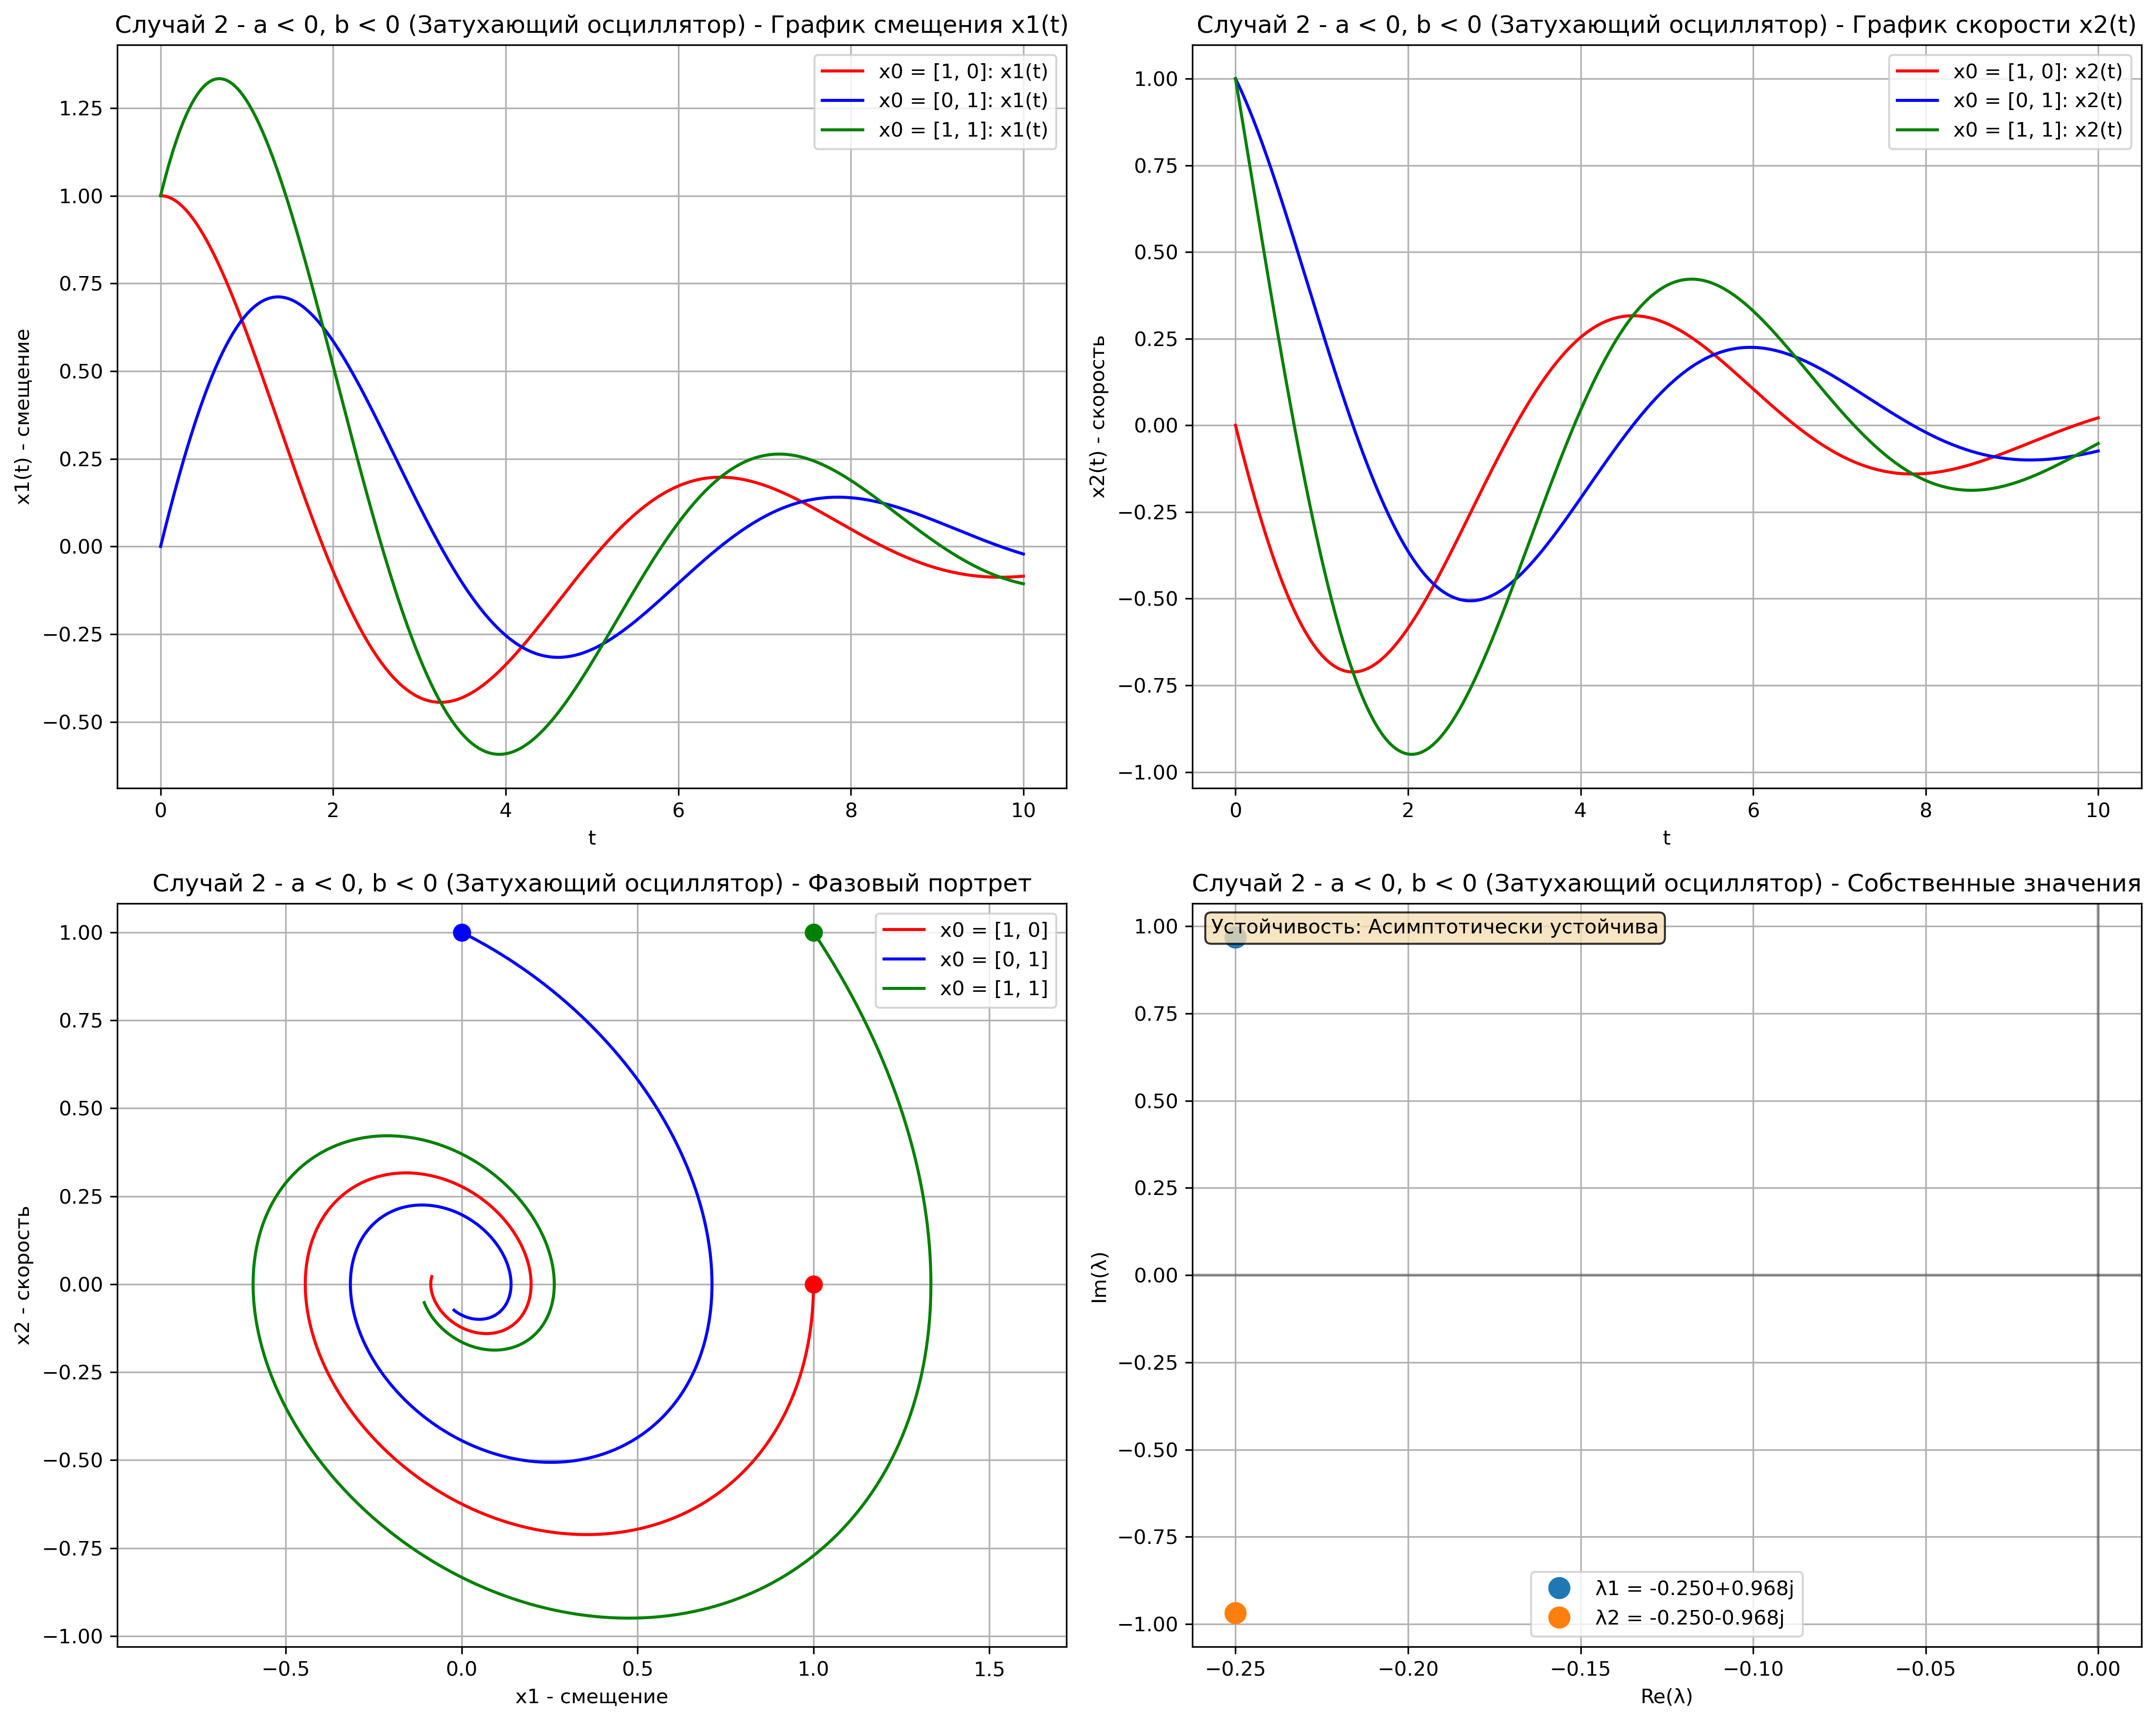
\includegraphics[width=0.8\textwidth]{images/task3/случай_2_-_a_<_0_b_<_0_затухающий_осциллятор.png}
\caption{Случай 2: Затухающий гармонический осциллятор}
\label{fig:oscillator2}
\end{figure}

\subsection{Случай 3: $a > 0$, $b = 0$}

Физическая интерпретация: Неустойчивый осциллятор (например, маятник в перевернутом положении).

$x_1$ - смещение от неустойчивого положения равновесия
$x_2$ - скорость
$a$ - коэффициент упругости (положительный - неустойчивость)
$b$ - коэффициент затухания (равен нулю)

Собственные значения: $\lambda_{1,2} = \pm \sqrt{a}$

Система неустойчива.

\begin{figure}[h!]
\centering
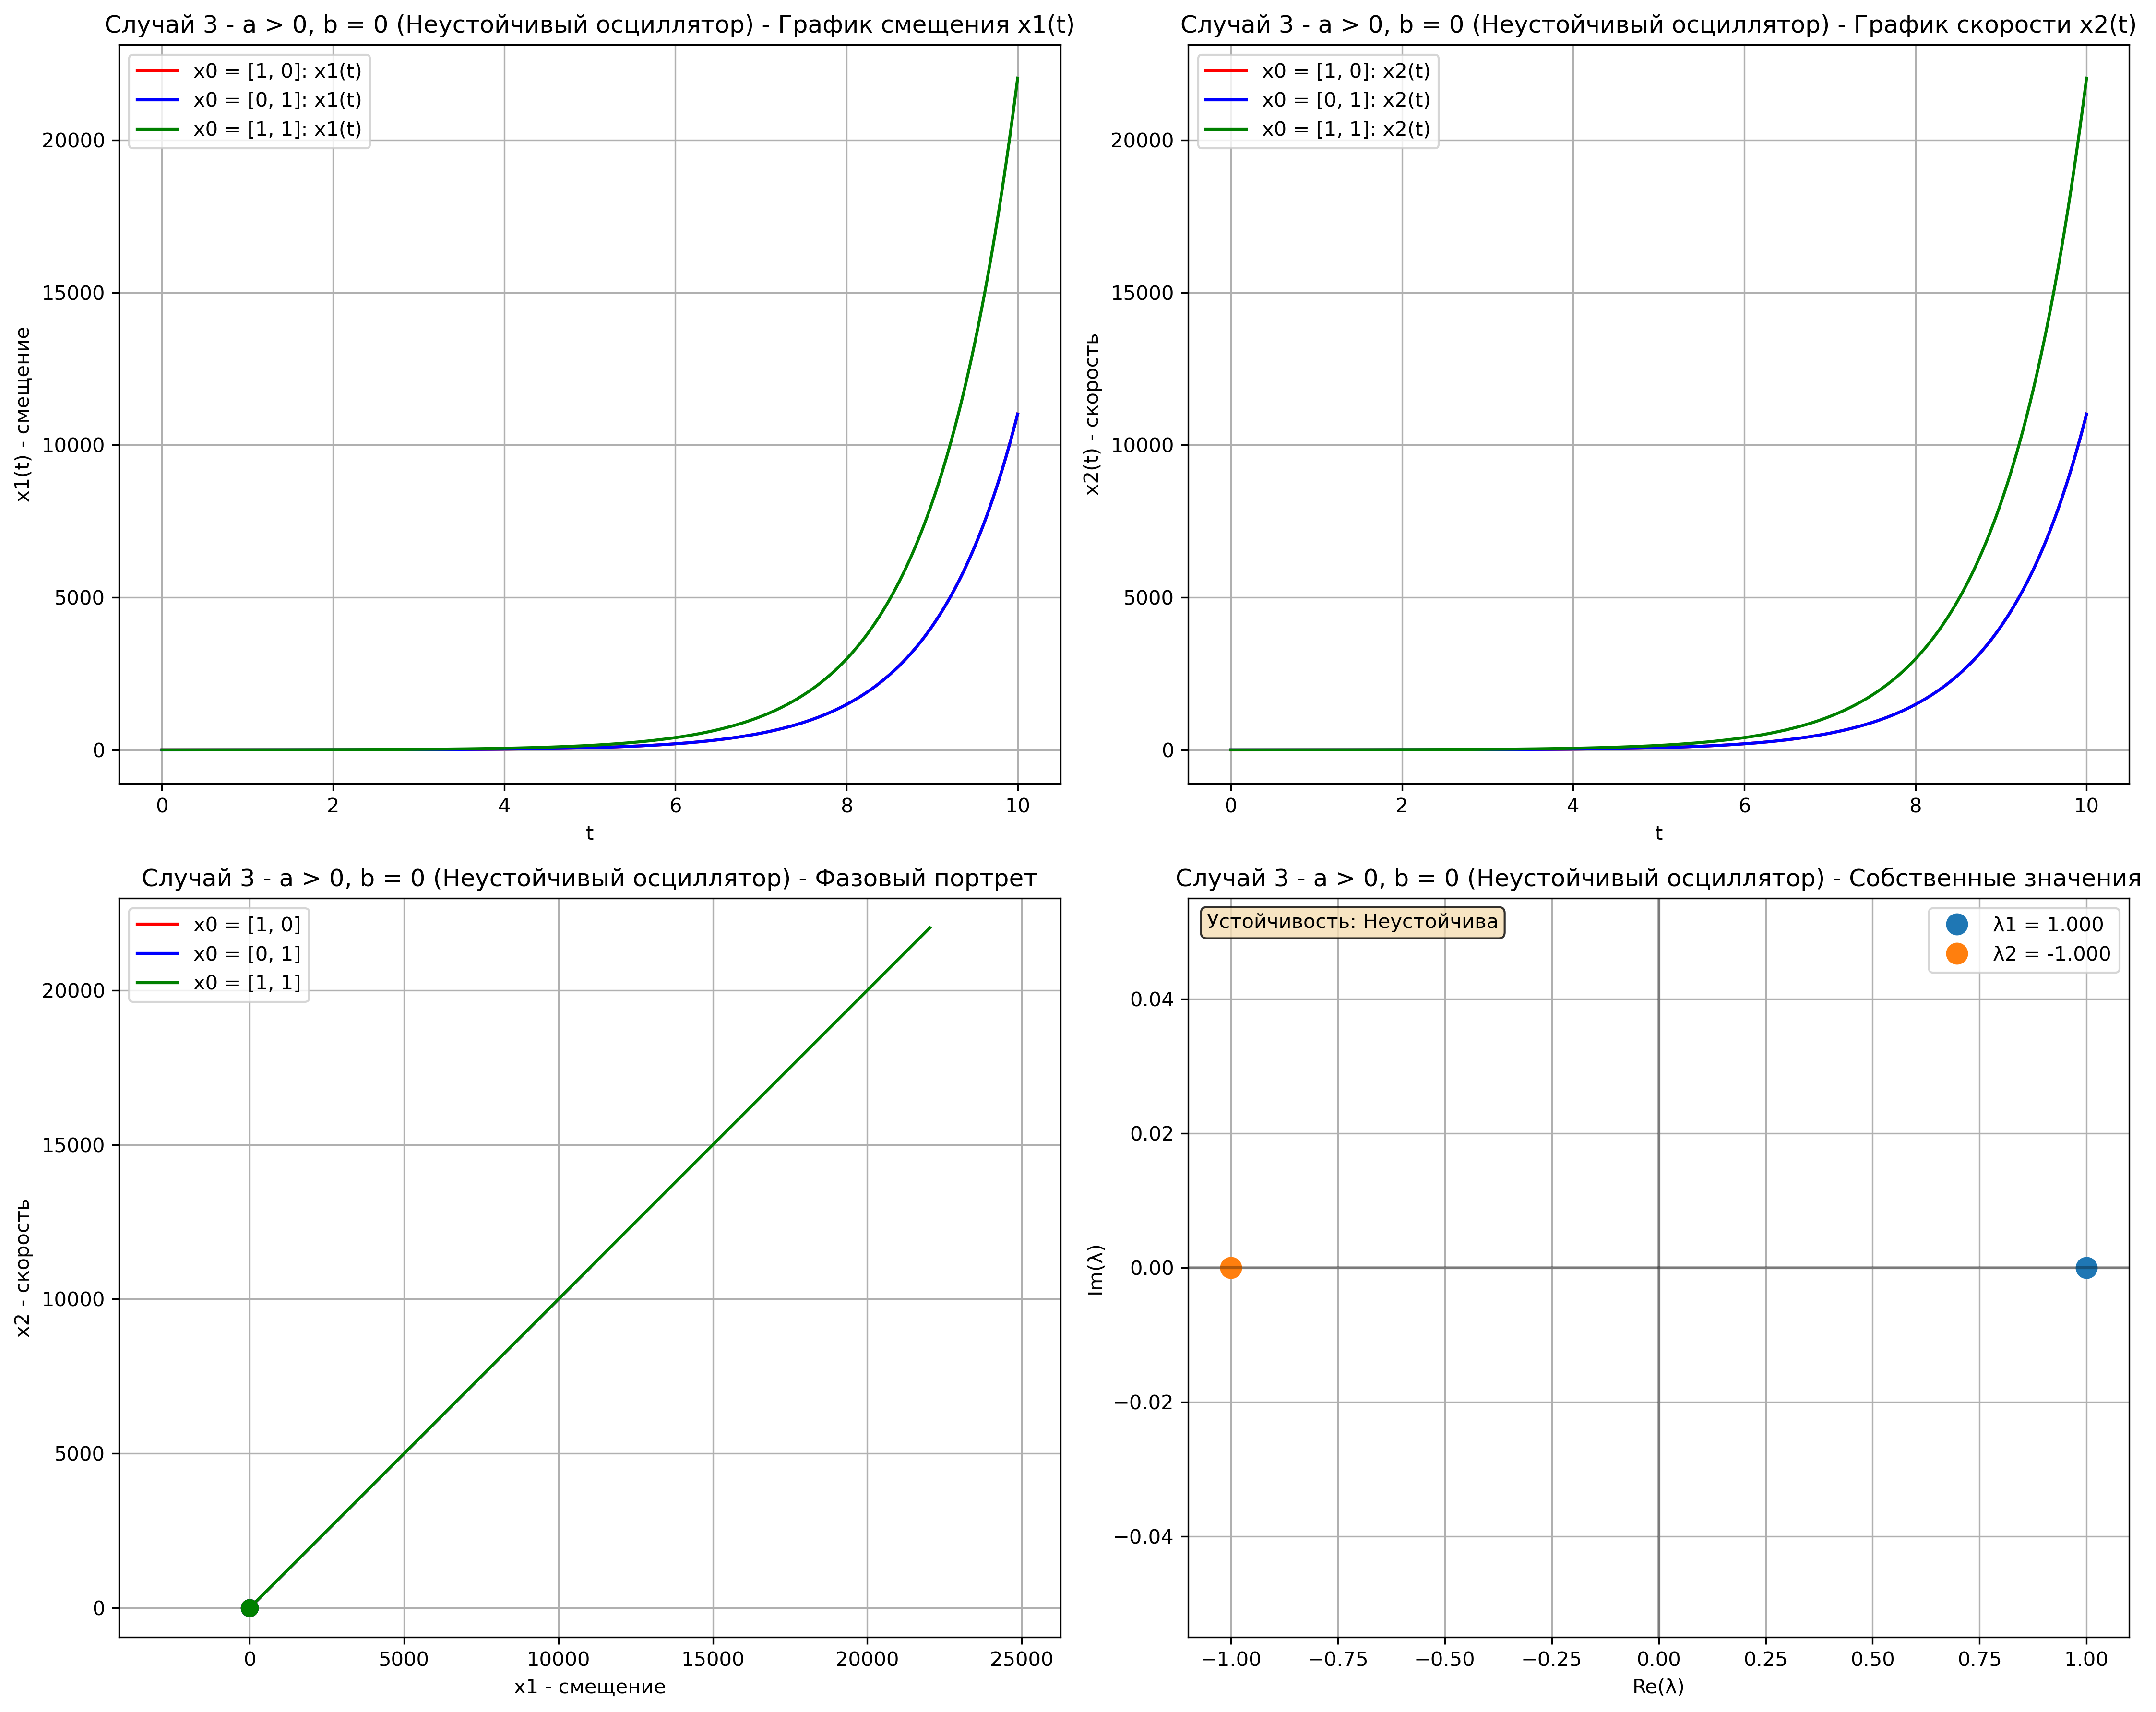
\includegraphics[width=0.8\textwidth]{images/task3/случай_3_-_a_>_0_b_=_0_неустойчивый_осциллятор.png}
\caption{Случай 3: Неустойчивый осциллятор}
\label{fig:oscillator3}
\end{figure}

\subsection{Случай 4: $a > 0$, $b < 0$}

Физическая интерпретация: Неустойчивый осциллятор с затуханием.

$x_1$ - смещение от неустойчивого положения равновесия
$x_2$ - скорость
$a$ - коэффициент упругости (положительный - неустойчивость)
$b$ - коэффициент затухания (отрицательный)

Одно собственное значение положительное, другое отрицательное.

Система неустойчива.

\begin{figure}[h!]
\centering
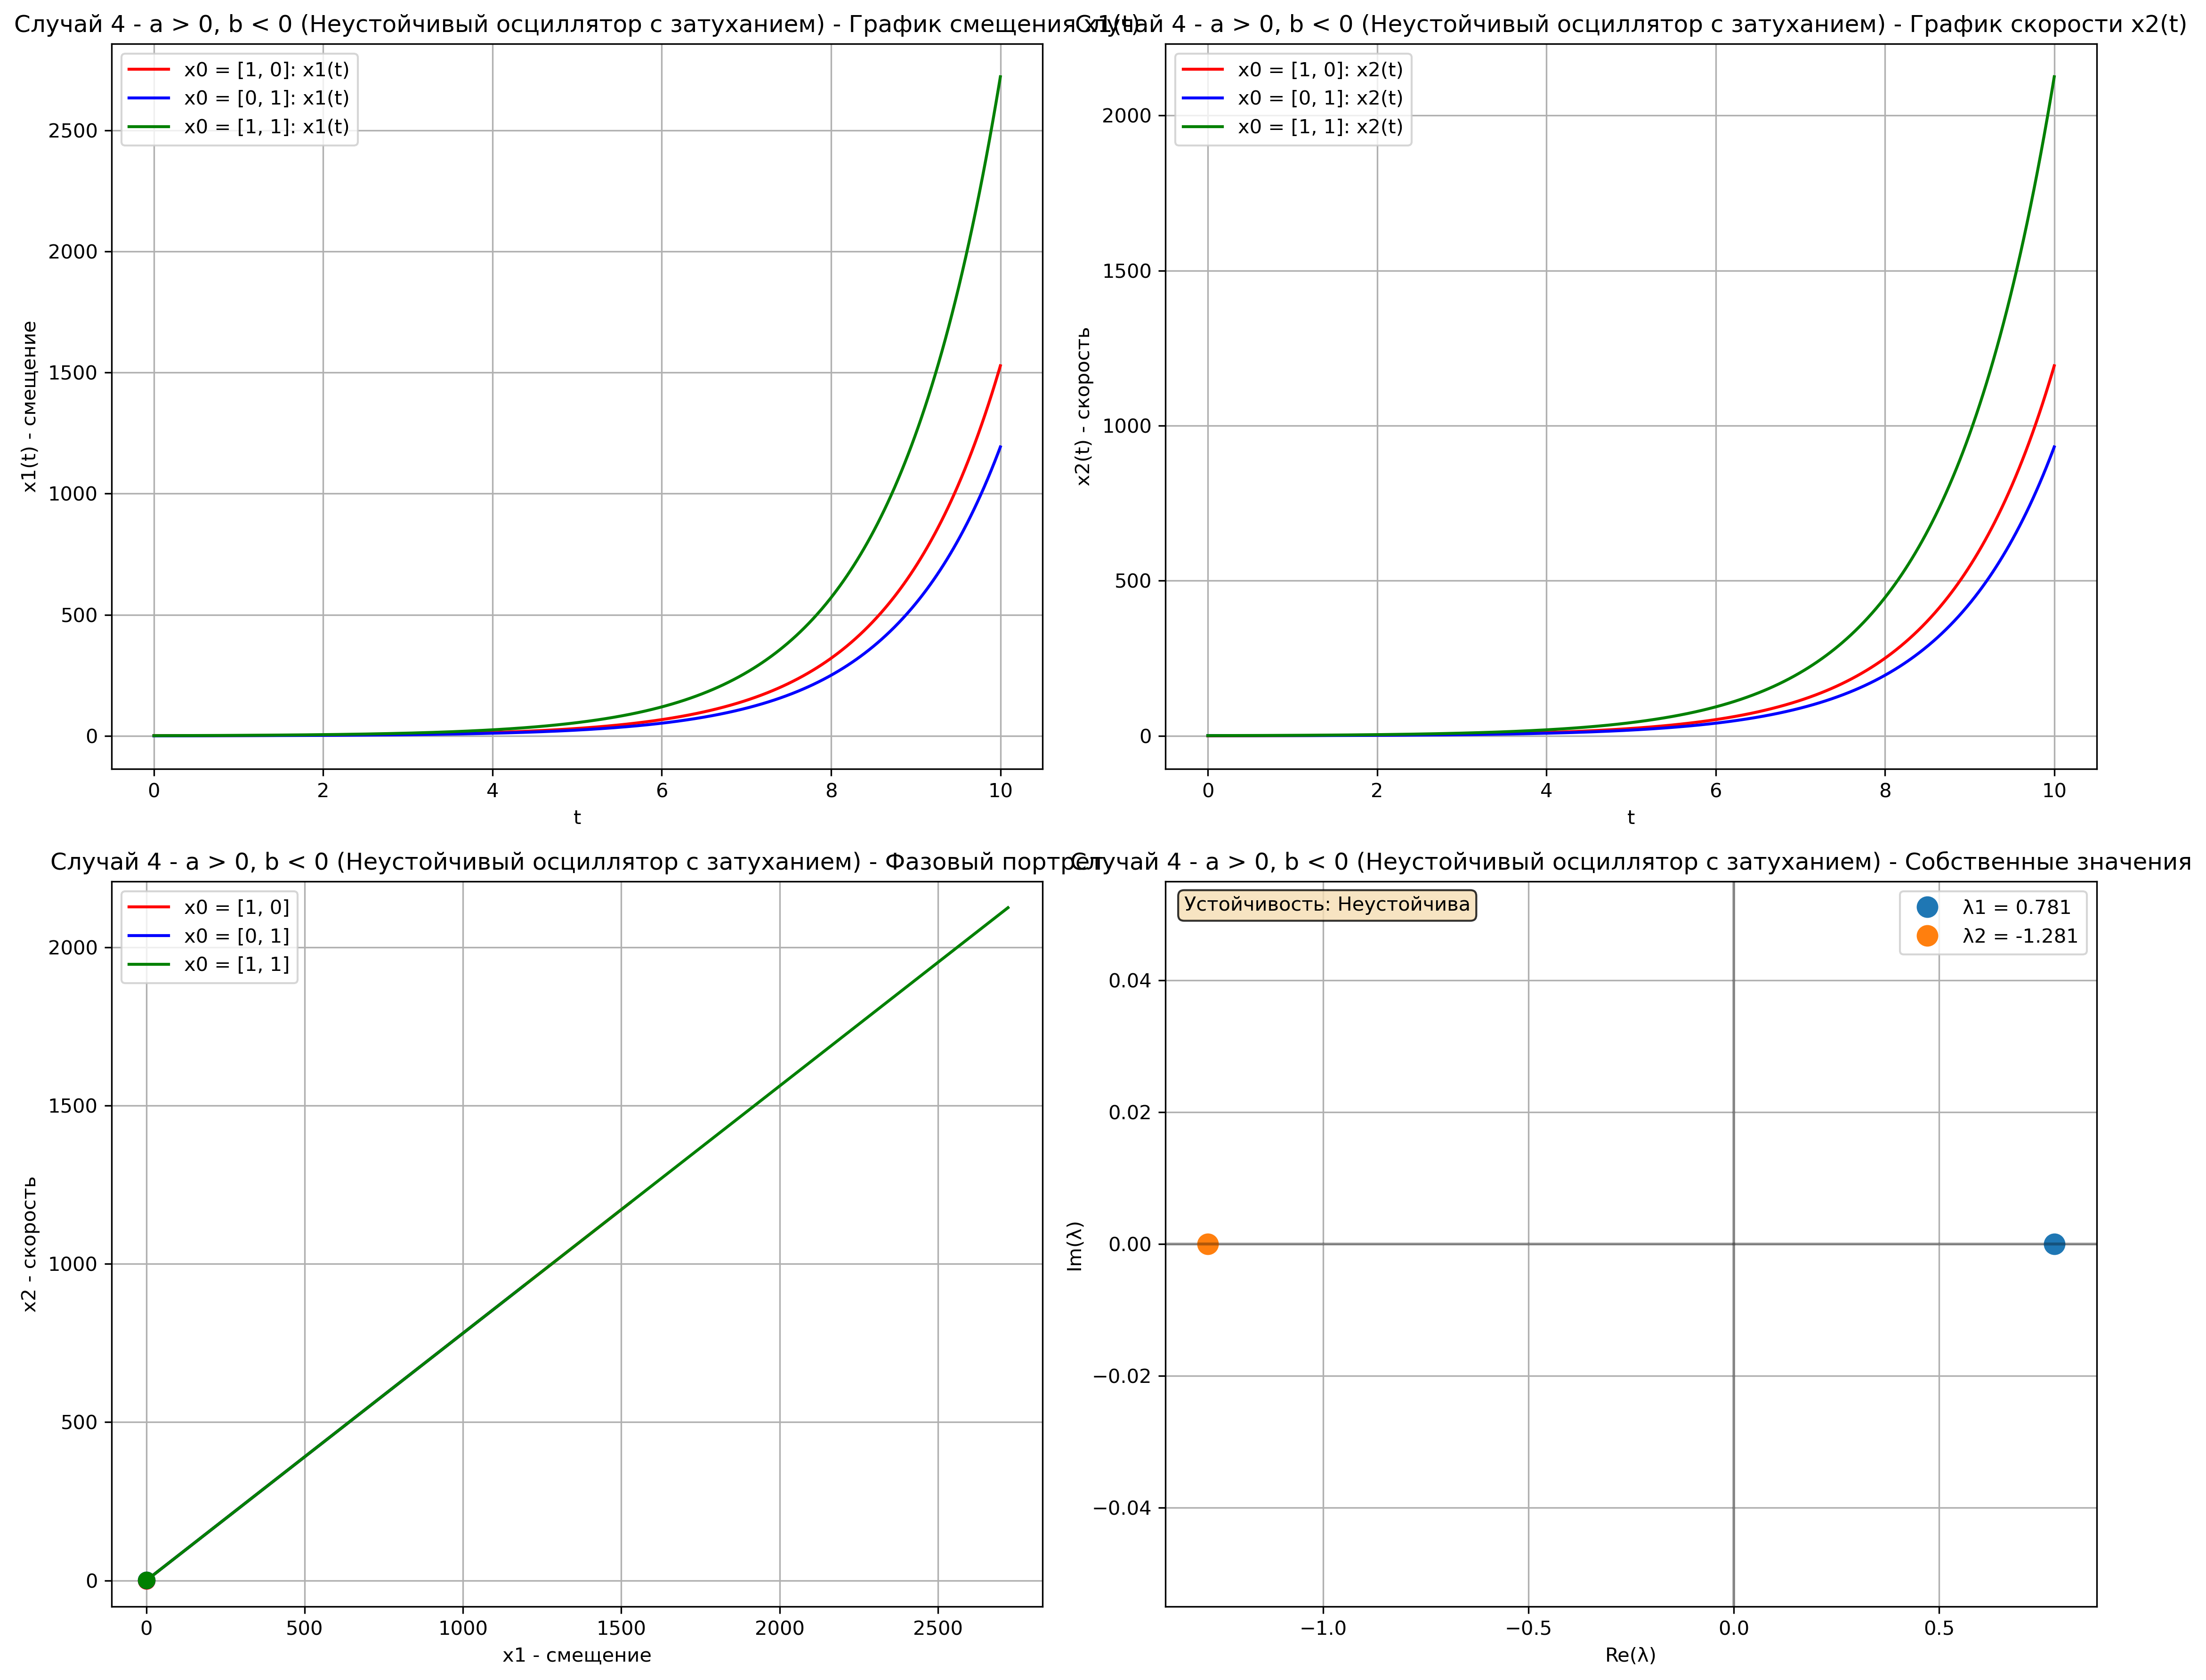
\includegraphics[width=0.8\textwidth]{images/task3/случай_4_-_a_>_0_b_<_0_неустойчивый_осциллятор_с_затуханием.png}
\caption{Случай 4: Неустойчивый осциллятор с затуханием}
\label{fig:oscillator4}
\end{figure}

\section{Выводы}

В ходе выполнения лабораторной работы были исследованы различные типы динамических систем:

\begin{enumerate}
\item \textbf{Непрерывные системы}: Изучены системы с различными типами устойчивости - асимптотически устойчивые, неустойчивые и нейтрально устойчивые. Показано влияние собственных значений и собственных векторов на поведение системы.

\item \textbf{Дискретные системы}: Исследованы системы с различными расположениями собственных значений на комплексной плоскости. Показано, что расположение собственных значений относительно единичной окружности определяет характер движения системы.

\item \textbf{Осциллятор}: Проанализирована система осциллятора с различными параметрами. Показана связь между физическими параметрами системы и её математическими свойствами устойчивости.
\end{enumerate}

Полученные результаты демонстрируют важность анализа собственных значений для понимания поведения динамических систем и их устойчивости.
